%%%%%%%%%%%%%%%%%%%%%%%%%%%%%%%%%%%%%%%%%%%%%%%%%%%%%%%%%%%%%%%%%%%%%%%%%%%%%%
% ASU Dissertation Template
%%%%%%%%%%%%%%%%%%%%%%%%%%%%%%%%%%%%%%%%%%%%%%%%%%%%%%%%%%%%%%%%%%%%%%%%%%%%%%
% Copyright 2021 Robert W. Kutter (robert@kutterconsulting.com)
%
%   See also: http://kutterconsulting.com
%
% For guidance on using this file, see the README.
%
%%%%%%%%%%%%%%%%%%%%%%%%%%%%%%%%%%%%%%%%%%%%%%%%%%%%%%%%%%%%%%%%%%%%%%%%%%%%%%
% Preamble
%%%%%%%%%%%%%%%%%%%%%%%%%%%%%%%%%%%%%%%%%%%%%%%%%%%%%%%%%%%%%%%%%%%%%%%%%%%%%%
\newcommand*{\pointsize}{12pt}          %<Set the font size; make sure the size is correct
                                        %   for the font you will use
\documentclass[letterpaper,             % Use US letter-size paper
               oneside,                 % No verso and recto differences
               \pointsize]              % Uses the font size defined above
               {memoir}
\renewcommand{\cleardoublepage}%        % \cleardoublepage will create entirely blank
  {\clearpage}%                         %   pages depending on settings (e.g., usually
                                        %   before start of \mainmatter); redefine it here
                                        %   so that no entirely blank pages are created
                                        %   automatically
%%%%%%%%%%%%%%%%%%%%%%%%%%%%%%%%%%%%%%%
% (Some) Packages
%%%%%%%%%%%%%%%%%%%%%%%%%%%%%%%%%%%%%%%
\usepackage{graphicx}                   % For importing image files
\usepackage{etoolbox}                   % For advanced commands throughout preamble
\usepackage{microtype}                  %~Improves kerning and protrusion (optional);
                                        %   See here for an introduction:
                                        %   http://www.khirevich.com/latex/microtype/

\providetoggle{usemicrotype}            % TRUE = microtype is being used
\makeatletter                           %   (Used to turn of microtype protrusion in the
\@ifpackageloaded{microtype}%           %   table of contents.)
  {\settoggle{usemicrotype}{true}}%
  {\settoggle{usemicrotype}{false}}
\makeatother
\usepackage{changepage}                 % For changing page layout (e.g., margins) in the
                                        %   middle of the document
\usepackage{calc}					              % Calculate text widths; used in page layout
                                        %   changes

%%%%%%%%%%%%%%%%%%%%%%%%%%%%%%%%%%%%%%%
% Title page, input
%%%%%%%%%%%%%%%%%%%%%%%%%%%%%%%%%%%%%%%
\listadd{\titlelines}%
  {First Line of the Title}             %<Enter the title of the dissertation
\listadd{\titlelines}%
  {Second Line of the Title}            % If you want to
                                        %   split the title across lines,
                                        %   use another \listadd command for the
                                        %   second line
\newcommand*\Author{Your Name}          %<Enter your name; must match official transcript
\newcommand*{\documentname}%
  {Dissertation}                        %<Enter the type of document (capitalized)
\newcommand*{\degreename}
  {Doctor of Philosophy}                %<Enter the type of degree (capitalized)
\newcommand*\defdate{April 2021}        %<Give month (written out fully) and year of
                                        %   the oral defense
\listadd{\committeechair}{Chair Name}   %<Enter committee chair name; use \listadd for
%\listadd{\committeechair}{Another name}%   for additional names
\newcommand*{\chairlabel}{Chair}        %<If you have co-chairs, replace this text with
                                        %   'Co-Chair'
\listadd{\committeemember}{Member Name} %<Enter committee member names; use \listadd for
\listadd{\committeemember}{Member Name} %   additional names
\newcommand*{\gradmonth}{May}           %<Enter the graduation date; month can only be:
                                        %  May, August, or December
\newcommand*{\gradyear}{2021}           %<Enter the graduation year, e.g. 2014

\listadd{\keywords}{keyword 1}          %<Enter keywords; use \listadd for
\listadd{\keywords}{keyword 2}          %   additional names (up to 6)
\newcommand*{\graddate}{\gradmonth%     % Compose full graduation date
  \space\gradyear}

%%%%%%%%%%%%%%%%%%%%%%%%%%%%%%%%%%%%%%%
% Page layout
%%%%%%%%%%%%%%%%%%%%%%%%%%%%%%%%%%%%%%%
\settrimmedsize{\stockheight}%          % Specifies \paperheight and \paperwidth
  {\stockwidth}{*}
\settrims{0pt}{0pt}                     % Set location of page in relation to the stock.
                                        % Paper and stock size are equivalent,
                                        % so both \trimtop and \trimedge are set to 0pt
\newlength{\forfootskip}
\setlength{\forfootskip}%
  {3\baselineskip}
\newlength{\textblockheight}            % Calculate height of text block to leave room
\setlength{\textblockheight}{9.0in}     %   for footers, keeping page numbers outside
\addtolength{\textblockheight}%         %   the 1in vertical margins
  {-\forfootskip}
\settypeblocksize{\textblockheight}%    % Calculated by 1.0in vertical margins and
  {*}{*}                                %   letting margins set the width of the typeblock
\setulmargins{1.0in}{*}{*}              % Set upper margin (\uppermargin, not \topmargin);
                                        %   calculate the bottom margin
\setlrmarginsandblock{1.25in}{1.25in}{*}%~Set margins and calculate width of typeblock
\setheaderspaces{*}{0.5\baselineskip}{*}% Arguments: '\headdrop', '\headsep', and/or ratio
                                        %   Note: This is only used in the list of
                                        %   contents sections
\setheadfoot{\baselineskip}%            % Set '\headheight' and '\footskip'
  {\forfootskip}
\checkandfixthelayout                   % Required by memoir package after setting layout
\settypeoutlayoutunit{in}               % Write layout dimensions to log file in inches

%%%%%%%%%%%%%%%%%%%%%%%%%%%%%%%%%%%%%%%
% Fonts
%%%%%%%%%%%%%%%%%%%%%%%%%%%%%%%%%%%%%%%
\usepackage[T1]{fontenc}                % Standard option to handle, e.g., accented
                                        %   characters like 'ö' better
\usepackage{amssymb,mathtools}          % For AMS-LaTeX, see here for more:
                                        %     http://www.ams.org/publications/authors/tex/amslatex
                                        % ('mathtools' loads and extends 'amsmath')
\usepackage{ifxetex,ifluatex}           % Can check if XeTeX or LuaTeX was used to typeset
\usepackage{fixltx2e}                   % Provides \textsubscript
\IfFileExists{upquote.sty}%             % Use upquote if available, for
  {\usepackage{upquote}}{}              %   straight quotes in verbatim environments

% Load fonts depending on the
%   typesetting engine
\ifnum 0\ifxetex 1\fi\ifluatex 1\fi=0   % If pdftex
  \usepackage[utf8]{inputenc}           %   'utf8' should match the encoding of this file
                                        %
                                        %~Set up your font in pdftex here
                                        %
\else 									                % If xetex or luatex
  \ifxetex                              % If xetex
    \usepackage{mathspec}               % Matches non-math open-type font to math
                                        %   open-type font (use 'mathspec' if you want to
                                        %   write math in unicode)
    \usepackage{xunicode}               % Convert LaTeX character macros to unicode
  \else                                 % If luatex\usepackage{fontspec}
    \usepackage{fontspec}               % Use fontspec for (open type) font selection
  \fi
  \defaultfontfeatures{Mapping=tex-text,% Font spec setting
    Scale=MatchLowercase}
  \newcommand*{\euro}{€}

  % Using fonts in XeLaTeX can be complicated; the following settings
  % work when this file is compiled inside the Docker container produced
  % by the `build.sh` script.
  %
  % Sometimes something simple like the following will work:
  %
  %   \setmainfont{Garamond}
  %
  % But often the easiest solution is to move font files (*.otf or *.ttf) into
  % a sub-directory and provide the direct path to them here.
  %
  % See `fontspec` documentation for more on using local font files.
  %
  \setmainfont{EBGaramond12}[           %<Set the main font; make sure the font is correct
                                        %   for the font size (See ASU Style Guide)
    Path          = /usr/share/fonts/opentype/ebgaramond/,
    Extension     = .otf ,
    UprightFont   = *-Regular ,
    ItalicFont    = *-Italic ,
    % Notice that bold is missing here because the Docker image does not have
    % a bold typeface for Garamond; it would probably be possible to find
    % one on your local system or online.
  ]

%  \setmathfont(Digits,Latin,Greek)%     %~Uncomment two lines to set a font for math%
%    {MATHFONT}
\fi

%%%%%%%%%%%%%%%%%%%%%%%%%%%%%%%%%%%%%%%
% Line spacing
%%%%%%%%%%%%%%%%%%%%%%%%%%%%%%%%%%%%%%%
\DoubleSpacing                          % True double spacing
\BeforeBeginEnvironment{quote}          % Memoir leaves most special material
  {\par\SingleSpacing}                  %   single spaced, but makes block quotes
\AfterEndEnvironment{quote}%            %   double-spaced; fix to follow ASU style guide
  {\vspace{-\baselineskip} %
  \DoubleSpacing}
\BeforeBeginEnvironment{quotation}%
  {\par\SingleSpacing}
\AfterEndEnvironment{quotation}%
  {\vspace{-\baselineskip} %
  \DoubleSpacing}

\setlength{\footnotesep}{\baselineskip} % Double space *between* footnotes
\renewcommand*{\footnoterule}{%         % Redefine footnoterule so that initial footnote
  \kern-3pt%                            %   still appears right under the rule (changing
  \hrule width 0.4\columnwidth          %   \footnotesep also changes the space between the
  \kern 2.6pt                           %   rule and the first footnote
  \vspace{-0.5\baselineskip}            % (Here is the vertical space adjustment)
  }

\usepackage{enumitem}                   % Control spacing in enumerate environment
\setlist{noitemsep}                     % Remove extra vertical spacing between items in lists
                                        % \setlist{nosep} to leave no space around whole list

%%%%%%%%%%%%%%%%%%%%%%%%%%%%%%%%%%%%%%%
% Page numbering
%%%%%%%%%%%%%%%%%%%%%%%%%%%%%%%%%%%%%%%
\makepagestyle{ASU}
  \makeevenfoot{ASU}{}{\thepage}{}
  \makeoddfoot{ASU}{}{\thepage}{}

%%%%%%%%%%%%%%%%%%%%%%%%%%%%%%%%%%%%%%%
% Title page, formatting
%%%%%%%%%%%%%%%%%%%%%%%%%%%%%%%%%%%%%%%
\newlength{\savedfootskip}
\setlength{\savedfootskip}{\footskip}
\newcommand{\titlepagesetup}{%          % Page layout for title page
  \changepage%                          % Adjustment to page dimensions:
    {\savedfootskip}%                   %   text height
    {}%                                 %   text width
    {}%                                 %   even-side margin
    {}%                                 %   odd-side margin
    {}%                                 %   column sep.
    {}%                                 %   topmargin
    {}%                                 %   headheight
    {}%                                 %   headsep
    {-\savedfootskip}%                  %   footskip
}

\newcommand{\closetitlepagesetup}{%     % Undo set up for title page
  \changepage{-\savedfootskip}{}{}{}{}%
    {}{}{}{\savedfootskip}%
}

\makeatletter                           % Do not modify this section; Enter info above
\newcommand*{\titlepageASU}{
  \titlepagesetup
  \clearpage
  \begin{center}
  \SingleSpacing
  \thispagestyle{empty}
    \renewcommand*{\do}[1]{##1 \\[\baselineskip]}
    \dolistloop{\titlelines}
    by \\[\baselineskip]
    \Author \\[5\baselineskip]
    A \documentname~Presented in Partial Fulfillment \\
    of the Requirements for the Degree \\
    \degreename \\
    \vfill                              % Vertically center the portion below
    Approved \defdate~by the \\
    Graduate Supervisory Committee: \\[\baselineskip]
    \renewcommand*{\do}[1]{##1, \chairlabel \\}
    \dolistloop{\committeechair}
    \renewcommand*{\do}[1]{##1 \\}
    \dolistloop{\committeemember}
    \vfill                              % Vertically center the portion above
    ARIZONA STATE UNIVERSITY \\[\baselineskip]
    \graddate
  \end{center}
  \clearpage
  \closetitlepagesetup
}
\makeatother

%%%%%%%%%%%%%%%%%%%%%%%%%%%%%%%%%%%%%%%
% Heading styles
%%%%%%%%%%%%%%%%%%%%%%%%%%%%%%%%%%%%%%%
% Note: memoir also has \book and \part commands; do not use these
\makechapterstyle{ASU}{%                % Define chapter heading style
  \renewcommand*{\chapterheadstart}{}   % Chapter title flush with top margin
  \renewcommand*{\chapnamefont}%        % Set font for 'Chapter' or 'Appendix'
    {\normalfont}
  \renewcommand*{\chapnumfont}%         % Set font for number in chapter headings
    {\normalfont}
  \renewcommand*{\afterchapternum}%     % Insert a double line break after
    {\\[\baselineskip]}                 %   chapter number
  \renewcommand*{\chaptitlefont}%       % Set font for chapter title name
    {\normalfont}
  \setlength{\afterchapskip}{0pt}       % Set vertical space between chapter title and
                                        %   first paragraph; equivalent to one line break
                                        %   (vertical space = \afterchapskip + \baselineskip)
                                        % Note: This \afterchapskip value is only used in
                                        %   front matter
  \renewcommand*{\printchapternum}{%    % Center justify chapter number
    \centering \chapnumfont %
    \thechapter}
  \renewcommand*{\printchaptertitle}[1]%% Center justify
    {\expandafter\centering %           %   \MakeUppercase has issues; see here for some
    \expandafter\chaptitlefont %        %   details: https://tex.stackexchange.com/questions/35680/uppercase-in-newcommand
    \expandafter\MakeUppercase %        %   Accented characters and some fonts may not
    \expandafter{##1}}                  %   uppercase correctly; if that happens, just
                                        %   type the chapter title in uppercase
}

\setsecnumdepth{all}                    %~Enter the levels that you want to have numbered
                                        %   (Default is to number all [5 levels deep].)

\newcommand{\divisionbeforeskip}%       % Create default formatting for headings
  {\baselineskip}
\newcommand{\divisionindent}%
  {0.5em}
\newcommand{\divisionfont}{\normalfont} % Font must be \normalfont
\newcommand{\divisionafterskip}%
  {\baselineskip}

\setbeforesecskip{\divisionbeforeskip}  % Apply default formatting to all heading levels
\setsecindent{\divisionindent}          % Note: If you change \setsecnumdepth above, you
\setsecheadstyle{\divisionfont}         %   will need to set the indent for all lower
\setaftersecskip{\divisionafterskip}    %   levels to '0pt'; otherwise, they will be
                                        %   preceded by unnecessary space
\setbeforesubsecskip{\divisionbeforeskip}
\setsubsecindent{\divisionindent}
\setsubsecheadstyle{\divisionfont}
\setaftersubsecskip{\divisionafterskip}

\setbeforesubsubsecskip{\divisionbeforeskip}
\setsubsubsecindent{\divisionindent}
\setsubsubsecheadstyle{\divisionfont}
\setaftersubsubsecskip{\divisionafterskip}

\setbeforeparaskip{\divisionbeforeskip}
\setparaindent{\divisionindent}
\setparaheadstyle{\divisionfont}
\setafterparaskip{\divisionafterskip}

\setbeforesubparaskip{\divisionbeforeskip}
\setsubparaindent{\divisionindent}
\setsubparaheadstyle{\divisionfont}
\setaftersubparaskip{\divisionafterskip}

%%%%%%%%%%%%%%%%%%%%%%%%%%%%%%%%%%%%%%%
% Paragraph formatting
%%%%%%%%%%%%%%%%%%%%%%%%%%%%%%%%%%%%%%%
%\sloppybottom                          % Reduce the chances of widows
\raggedbottom                           % Loosens vertical spacing requirements, so
                                        %   \sloppybottom doesn't make pages look bad;
                                        %   it also prevents large gaps in the middle of
                                        %   pages and pushes them to the bottom of pages
\indentafterchapter                     % Overrides the default which is not to indent
                                        %   the first paragraph in a chapter, but it
                                        %   looks odd in some places to not indent
                                        %   paragraphs

%%% List Titles %%%
\renewcommand{\contentsname}%           % Set heading for each list
  {Table of Contents}%                  %   Formatted as chapter headings by default, so
\renewcommand{\listtablename}%          %   no additional heading formatting is needed
  {List of Tables}
\renewcommand{\listfigurename}%
  {List of Figures}

%%% Depth %%%
\settocdepth{subparagraph}              % Include 5 levels deep (all levels) in TOC

%%% Fonts %%%
\makeatletter%
\patchcmd{\l@part}%                     % Patch the command that writes part-level entries
    {\cftpartfont {#1}}%                %   to the table of contents, so they are in
    {\normalfont \texorpdfstring{%      %   'normalfont' and uppercase
      \uppercase{#1}}{{#1}} }%
    {\typeout{Success: Patch %
      'l@part' to uppercase %
      part-level headings in the %
      table of contents.}}%
    {\typeout{Fail: Patch %
      'l@part' to uppercase %
      part-level headings in the %
      table of contents.}}%
\makeatother%

\makeatletter%
\patchcmd{\l@chapapp}%                  % Patch the command that writes chapter-level
    {\cftchapterfont {#1}}%             %   entries to the table of contents, so they are
    {\normalfont \texorpdfstring{%      %   in 'normalfont' and uppercase
      \uppercase{#1}}{{#1}} }%
    {\typeout{Success: Patch %
      'l@chapapp' to uppercase %
      part-level headings in the %
      table of contents.}}%
    {\typeout{Fail: Patch %
      'l@chapapp' to uppercase %
      part-level headings in the %
      table of contents.}}%
\makeatother%

% If not using 'hyperref', use the following commands to adjust 'part' and 'chapter'
%   level headings in the TOC
%\renewcommand*{\cftpartfont}%          % Uppercase 'part' and 'chapter' headings
%  {\normalfont\MakeTextUppercase}      % Note: Sending \MakeTextUppercase to the TOC
%\renewcommand*{\cftchapterfont}%       %   conflicts with hyperref and breaks it!
%  {\normalfont\MakeTextUppercase}%

\usepackage{titlecaps}                  % Set up headline style for captions in the
                                        %   lists of tables and figures
                                        % Note: ASU style guide does not provide
                                        %   comprehensive guidelines for headlines, so
                                        %   Chicago style for headline style is used
                                        % Note: Last word in title is not explicitly
                                        %   capitalized; in general, these settings are
                                        %   broadly correct, but captions should be
                                        %   reviewed to ensure they are being capitalized
                                        %   properly
\Resetlcwords
\Addlcwords{a an the}                   % Leave articles lowercase
\Addlcwords{and but for or nor}         % Leave conjunctions lowercase
\Addlcwords{aboard about above across % % Leave all prepositions lowercase
  after against along amid among anti % %   (This is a [non-exhaustive] list of common
  around as at before behind below %    %   one-word prepositions)
  beneath beside besides between %
  beyond but by concerning considering %
  despite down during except excepting %
  excluding following for from in %
  inside into like minus near of off %
  on onto opposite outside over past %
  per plus regarding round save since %
  than through to toward towards under %
  underneath unlike until up upon %
  versus vs via with within without}
\Addlcwords{ according\space{to} %      % Leave two-word conjunctions lowercase
  ahead\space{of} apart\space{from} %   %   (This is a [non-exhaustive] list of common
  as\space{for} as\space{of} %          %   two-word prepositions.)
  as\space{per} as\space{regards} %
  aside\space{from} astern\space{of} %
  back\space{to} because\space{of} %
  close\space{to} due\space{to} %
  except\space{for} far\space{from} %
  in\space{to} inside\space{of} %
  instead\space{of} left\space{of} %
  near\space{to} next\space{to} %
  on\space{to} opposite\space{of} %
  opposite\space{to} out\space{from} %
  out\space{of} outside\space{of} %
  owing\space{to} prior\space{to} %
  pursuant\space{to} rather\space{than} %
  regardless\space{of} right\space{of} %
  subsequent\space{to} such\space{as} %
  thanks\space{to} that\space{of} %
  up\space{to}}

\renewcommand{\cfttableaftersnumb}%     % Put table captions in List of Tables in title
  {\titlecap}%                          %   case
\renewcommand{\cftfigureaftersnumb}%    % Put table captions in List of Figures in title
  {\titlecap}%                          %   case

\renewcommand*{\cftpartpagefont}%       % Use normal font for all page numbers
  {\normalfont}
\renewcommand*{\cftchapterpagefont}%
  {\normalfont}
\renewcommand*{\cftsectionpagefont}%
  {\normalfont}
\renewcommand*{\cftsubsectionpagefont}%
  {\normalfont}
\renewcommand*{\cftsubsubsectionpagefont}%
  {\normalfont}
\renewcommand*{\cftsubsubsectionpagefont}%
  {\normalfont}
\renewcommand*{\cftparagraphpagefont}%
  {\normalfont}
\renewcommand*{\cftsubparagraphpagefont}%
  {\normalfont}
\renewcommand*{\cftfigurepagefont}%
  {\normalfont}
\renewcommand*{\cfttablepagefont}%
  {\normalfont}

\cftpagenumbersoff{part}                % Turn off page numbers for 'part's, which are
                                        %   actually serving as headings within the TOC

%%% Vertical Space %%%
\setlength{\cftbeforepartskip}{0pt}     % Remove all additional vertical spacing so TOC
\setlength{\cftbeforechapterskip}{0pt}  %   is double spaced uniformly
\setlength{\cftbeforesectionskip}{0pt}
\setlength{\cftbeforesubsectionskip}{0pt}
\setlength{\cftbeforesubsubsectionskip}{0pt}
\setlength{\cftbeforeparagraphskip}{0pt}
\setlength{\cftbeforesubparagraphskip}{0pt}
\setlength{\cftbeforefigureskip}{0pt}
\setlength{\cftbeforetableskip}{0pt}

\renewcommand{\insertchapterspace}{%    % By default, extra vertical space (10pt) is
  \addtocontents{lof}%                  %   inserted between tables and figures from
    {\protect\addvspace{0pt}}%          %   different chapters; remove this extra space.
  \addtocontents{lot}%
    {\protect\addvspace{0pt}}%
}

%%% Horizontal Space %%%
\newlength{\levelindentincrement}       % Set indent to increase by the same amount for
\setlength{\levelindentincrement}{2em}  %   each level in the TOC; don't adjust figure
\newlength{\levelindent}                %   or table indents
\setlength{\levelindent}%
  {\levelindentincrement}
\setlength{\cftchapterindent}%
  {\levelindent}
\addtolength{\levelindent}%
  {\levelindentincrement}
\setlength{\cftsectionindent}%
  {\levelindent}
\addtolength{\levelindent}%
  {\levelindentincrement}
\setlength{\cftsubsectionindent}%
  {\levelindent}
\addtolength{\levelindent}%
  {\levelindentincrement}
\setlength{\cftsubsubsectionindent}%
  {\levelindent}
\addtolength{\levelindent}%
  {\levelindentincrement}
\setlength{\cftparagraphindent}%
  {\levelindent}
\addtolength{\levelindent}%
  {\levelindentincrement}
\setlength{\cftsubparagraphindent}%
  {\levelindent}
\addtolength{\levelindent}%
  {\levelindentincrement}

\setlength{\cftchapternumwidth}%        % Decrease space between number and heading for
  {0.85\cftchapternumwidth}             %   all heading levels
\setlength{\cftsectionnumwidth}%
  {0.85\cftsectionnumwidth}
\setlength{\cftsubsectionnumwidth}%
  {0.85\cftsubsectionnumwidth}
\setlength{\cftsubsubsectionnumwidth}%
  {0.85\cftsubsubsectionnumwidth}
\setlength{\cftparagraphnumwidth}%
  {0.85\cftparagraphnumwidth}
\setlength{\cftsubparagraphnumwidth}%
  {0.85\cftsubparagraphnumwidth}

% Calculate the indent to the first
% character in table and figure
% captions.
% This is more complicated because the
% document automatically considers
% the total number of figures and
% tables and increases the indent to
% make room for longer numbers.
\newcounter{totfigures}                 % Collect the total number of figures
\newcounter{tottables}                  % Collect the total number of tables

\providecommand\totfig{}                % Retrieve the total number of figures
\providecommand\tottab{}                % Retrieve the total number of tables

\makeatletter
\AtEndDocument{%                        % Store the totals
  \addtocounter{totfigures}{%
    \value{figure}%
  }%
  \addtocounter{tottables}{%
    \value{table}%
  }%
  \immediate\write\@mainaux{%
    \string\gdef\string\totfig{%
      \number\value{totfigures}%
    }%
    \string\gdef\string\tottab{%
      \number\value{tottables}%
    }%
  }%
}
\makeatother

% The calculation that appears inside
% this block needs to be done as the
% the document is written, not in the
% preamble. `\pretocmd` makes this
% calculation happen right before
% `\listoffigures` is executed.
\usepackage{calculator}
\pretocmd{\listoffigures}{%
  % Calculate the number of digits in
  % the total number of figures
  %
  % Here is the algorithm:
  %   Floor(Log10(\number)) + 1
  \MAX{\totfig}{1}{\figurecount}
  \LOG[10]{\figurecount}{\tempAfig}%
  \FLOOR{\tempAfig}{\tempBfig}%
  \ADD{\tempBfig}{1}{\digitsinfig}%     % Number of digits in number of figs
  %
  % Calculate space factor for figures
  % The space factor is just one less
  % than the number of digits, but it
  % must be at least 0.
  %
  \SUBTRACT{\digitsinfig}{1}{\tempDfig}%
  \MAX{\tempDfig}{0}{\tempEfig}%
  \MULTIPLY{\tempEfig}{0.55}{%
    \figspacefactor%                    % Space factor for figures in LOF
  }%
  % Apply the space factor for figures
  \setlength{\cftfigurenumwidth}{%      % Figure has the same 'level' as
    \cftchapternumwidth%                % 'chapter' in the figure list, so
  }%                                    % make the number spacing the same as
                                        % for chapters unless there are more
  \addtolength{\cftfigurenumwidth}{%    % than 9 figures; in that case, add
    \figspacefactor em%                 % extra space (as calculated in
  }%                                    % `\figspacefactor`
}{}{}

% Same space calculation for tables
\pretocmd{\listoftables}{%
  % Calculate the number of digits in
  % the total number of tables
  \MAX{\tottab}{1}{\tablecount}
  \LOG[10]{\tablecount}{\tempAtab}%
  \FLOOR{\tempAtab}{\tempBtab}%
  \ADD{\tempBtab}{1}{\digitsintab}%     % Number of digits in number of tabs
  % Calculate space factor for tables
  \SUBTRACT{\digitsintab}{1}{\tempDtab}%
  \MAX{\tempDtab}{0}{\tempEtab}%
  \MULTIPLY{\tempEtab}{0.55}{%
    \tabspacefactor%                    % Space factor for tables in LOT
  }%
  % Apply the space factor for tables
  \setlength{\cfttablenumwidth}{%
    \cftchapternumwidth%
  }%
  \addtolength{\cfttablenumwidth}{%
    \tabspacefactor em%
  }%
}{}{}

%%% Leaders/dots %%%
\renewcommand*{\cftdotsep}{1.7}         % Set distance between dots for all heading levels
\renewcommand*{\cftchapterleader}%      % Turn on dots for 'chapter' level
  {\normalfont\cftdotfill{\cftdotsep}}
\makeatletter                           % Bring leader dots over to page number (no gap)
  \renewcommand{\@pnumwidth}{1.55em}    %~Manually adjust
  \renewcommand{\@tocrmarg}{2.55em}
\makeatother

\renewcommand{\cfttableaftersnum}{.}    % Period after number in LOT
\renewcommand{\cftfigureaftersnum}{.}   % Period after number in LOF

%%% Printing List Titles and Headers in Content Lists
% Table of Contents (TOC)
\copypagestyle{ASUtoc}{ASU}%            % Page style for regular page in TOC
  \makeevenhead{ASUtoc}%
    {\leftmark}{}{Page}
  \makeoddhead{ASUtoc}%
    {\leftmark}{}{Page}

\copypagestyle{ASUtocFirst}{ASU}%       % Custom page headers for first page of TOC
  \makeevenhead{ASUtocFirst}%           %    (print out the title)
    {}%
    {\printchaptertitle{\contentsname}}%
    {}
  \makeoddhead{ASUtocFirst}%
    {}%
    {\printchaptertitle{\contentsname}}%
    {}

\renewcommand{\tocheadstart}{}%         % Usually content list titles are printed like
                                        %   chapter headings; empty that formatting

\renewcommand{\printtoctitle}[1]{}%     % Don't print TOC title using default method;
                                        %   it will be output in the header

\renewcommand{\aftertoctitle}{%         % On the first page of the TOC, print out the
  \thispagestyle{ASUtocFirst}%          %   TOC title using a custom page style and print
  \hfill Page\par%                      %   the heading for the page below in the regular
  }%                                    %   textbox
                                        % Note: Need '\par' before lists; see here: https://tex.stackexchange.com/questions/49882/yet-another-perhaps-a-missing-item-error

% List of Tables (LOT)
\copypagestyle{ASUlot}{ASU}%            % Page style for regular page in list of tables
  \makeevenhead{ASUlot}{Table}{}{Page}
  \makeoddhead{ASUlot}{Table}{}{Page}

\copypagestyle{ASUlotFirst}{ASU}%       % Custom page headers for first page of list of
  \makeevenhead{ASUlotFirst}%           %   tables (print out the title)
    {}%
    {\printchaptertitle{\listtablename}}%
    {}
  \makeoddhead{ASUlotFirst}%
    {}%
    {\printchaptertitle{\listtablename}}%
    {}

\renewcommand{\lotheadstart}{}%         % Usually content list titles are printed like
                                        %   chapter headings; empty that formatting;

\renewcommand{\printlottitle}[1]{}%     % Don't print LOT title using default method;
                                        %   it will be output in the header

\renewcommand{\afterlottitle}{%         % On the first page of the list of tables, print
  \thispagestyle{ASUlotFirst}%          %   out the title using a custom page style and
  Table\hfill Page\par}%                %   print heading below in regular textbox

% List of Figures (LOF)
\copypagestyle{ASUlof}{ASU}
  \makeevenhead{ASUlof}{Figure}{}{Page}
  \makeoddhead{ASUlof}{Figure}{}{Page}

\copypagestyle{ASUlofFirst}{ASU}%       % Custom page headers for first page of list of
  \makeevenhead{ASUlofFirst}%           %   figures (print out the title)
    {}%
    {\printchaptertitle{\listfigurename}}%
    {}
  \makeoddhead{ASUlofFirst}%
    {}%
    {\printchaptertitle{\listfigurename}}%
    {}

\renewcommand{\lofheadstart}{}%         % Usually content list titles are printed like
                                        %   chapter headings; empty that formatting

\renewcommand{\printloftitle}[1]{}%     % Don't print LOF title using default method;
                                        %   it will be output in the header

\renewcommand{\afterloftitle}{%         % On the first page of the list of figures, print
  \thispagestyle{ASUlofFirst}%          %   out the title using a custom page style and
  Figure\hfill Page\par}                %   print heading below in regular textbox

%%% Page layout (dimensions) for Contents Lists
\newlength{\verticalpush}               % Set up to change page dimensions for the table
                                        %   of contents
                                        % Push everything down so all the content is still
                                        %   1in from the top of the page, including the
                                        %   header, so the header is available for titles
                                        %   on the first page of contents lists and then
                                        %   the headings on subsequent pages
\setlength{\verticalpush}%              % Calculate difference between \headdrop and the
  {1.0in - \headdrop}                   %   total upper margin (1in), so you can push
                                        %   the top of the header down into the textbox

\newcommand{\contentslistsetup}{%       % Set up for contents lists
  \changepage%                          % Adjustment to page dimensions:
    {-\baselineskip}%                   %   text height
    {}%                                 %   text width
    {}%                                 %   even-side margin
    {}%                                 %   odd-side margin
    {}%                                 %   column sep.
    {\verticalpush}%                    %   topmargin
    {}%                                 %   headheight
    {}%                                 %   headsep
    {-\verticalpush+\baselineskip}%     %   footskip
}

\newcommand{\closecontentslistsetup}{%  % Undo set up for contents lists
  \changepage{\baselineskip}{}{}{}{}%
    {-\verticalpush}{}{}{\verticalpush-\baselineskip}%
}

% Content lists can also be output directly. If the following command were used, all the
%   headings would have to be output manually (i.e., can't rely on any memoir macros for
%   formatting or setting in contents lists headings and lists). It would be best to
%   create a custom macro, such as '\customtoc', to output headings and content lists
%   following the style guide.
%
% \makeatletter
%   \@starttoc{toc}
% \makeatother

% These pages partly explain why it's difficult to use 'afterpage' to change page layout
%   settings (essentially, it's because everything inside \afterpage has a local scope).
%   If it were possible to use 'afterpage' in that way, the content lists would  be
%   easier to format. A new page layout could be called after the first page of each
%   content  list. Instead, use page marks to get the layout required by the style guide.
% https://tex.stackexchange.com/questions/97126/attempts-to-manually-change-linewidth-ignored-by-latex
% https://tex.stackexchange.com/questions/85729/page-styles-only-work-for-thispagestyle-under-afterpage

%%%%%%%%%%%%%%%%%%%%%%%%%%%%%%%%%%%%%%%
% Footnotes and Endnotes
%%%%%%%%%%%%%%%%%%%%%%%%%%%%%%%%%%%%%%%
\usepackage{chngcntr}                   % Modify counters (e.g., for figures, footnotes)
\counterwithout*{footnote}{chapter}     % Make footnote numbering continuous throughout

\providetoggle{useendnotes}
\settoggle{useendnotes}{true}           %<Set to 'true' if you want to use endnotes
\iftoggle{useendnotes}{%                % Use the command \pagenote to create endnotes
                                        %   in the running text. They will be collected
                                        %   and printed in a 'Notes' section at the end
                                        %   of the document

  \makepagenote                         % Required in preamble if using endnotes
  \continuousnotenums                   % Numbering does *not* reset after each chapter
  \renewcommand*{\pagenotesubhead}[3]{} % No subheads inside note list (default is to
                                        %   divide them by chapter)
  \renewcommand*{\notenuminnotes}[1]%   % Remove extra space between note number and note
    {\normalfont #1.}                   %   text
  \renewcommand{\postnoteinnotes}%      % Double space *between* notes
    {\par\vspace{\baselineskip}}
}{}                                     % Do nothing here if not using endnotes

%%%%%%%%%%%%%%%%%%%%%%%%%%%%%%%%%%%%%%%
% Bibliography
%%%%%%%%%%%%%%%%%%%%%%%%%%%%%%%%%%%%%%%
\newcommand{\bibfilename}{%             %<Enter the name of the *.bib file containing the
  src/sample/library%                   %   reference information for sources cited in
}%                                      %   the text. God help you if you're doing
                                        %   citations manually.

\newcommand{\bibheading}{References}    %<Enter the heading for the references section:
                                        %   'References', 'Works Cited', or 'Bibliography'

\providetoggle{usebiblatex}             % True = a biblatex package is being used;
                                        %   False = 'natbib' is being used
\settoggle{usebiblatex}{true}           %~Set to 'false' to use 'natbib' intead of
                                        %   biblatex; I strongly recommend using biblatex
                                        %   because natbib is rather old and will break
                                        %   for innocuous things like underscores in URLs
\iftoggle{usebiblatex}{%                % Settings for citation package
%                                       % Settings for 'biblatex' or a version of
%                                       %   'biblatex'
  \usepackage[authordate,%
              backend=biber,%           % Recommend to use 'biber' instead of 'bibtex'
              doi=only,%                % Avoid printing URLs
              isbn=false]%              % Don't print ISBN numbers
              {biblatex-chicago}        %~Other possibilities include: 'biblatex',
                                        %   'biblatex-apa', and 'biblatex-mla'
  \bibliography{\bibfilename}
  \setlength{\bibitemsep}%              % Set vertical distance between
    {0.5\baselineskip}%                 %   bibliography entries
  \setcounter{biburlnumpenalty}{9000}   % Break URLs in bibliography across lines
  \setcounter{biburlucpenalty}{9000}
  \setcounter{biburllcpenalty}{9000}

  \usepackage[style=american,%          % Settings for quotation marks; load after
    english=american]{csquotes}%        %   'inputenc'; only use with biblatex; throws
  \MakeOuterQuote{"}%                   %   error when used with natbib
}{%                                     % Settings for 'natbib'
  \usepackage{natbib}%
  \newcommand{\natbibstyle}{%           %~Enter the name of the *.bst file to use to
    src/asudis%                         %   format citations with natbib. Default is
  }%                                    %   'asudis'. I do not know where 'asudis' came
                                        %   from, but apparently it formats citations
                                        %   correctly because it was included with the
                                        %   previous LaTeX template.
}

%%%%%%%%%%%%%%%%%%%%%%%%%%%%%%%%%%%%%%%
% Tables and figures
%%%%%%%%%%%%%%%%%%%%%%%%%%%%%%%%%%%%%%%
\captiondelim{. }                       %~Use period (.) after caption number instead of
                                        %   colon (:). Change according to style guide.
\captionstyle[\raggedright]%            % Set justifcation for [one line captions]
  {\raggedright}                        %   and {multiple line captions}
\setlength{\belowcaptionskip}{0pt}      % Bring caption down closer to figure/table
\makeatletter                           % Consecutive numbering throughout
  \counterwithout{figure}{chapter}      %   (including back matter)
  \counterwithout{table}{chapter}
  \renewcommand\@memfront@floats{}
  \renewcommand\@memmain@floats{}
  \renewcommand\@memback@floats{}
\makeatletter

\newcommand{\macrocapwrap}[1]{%         % Use this macro to place other macros inside
  {\bgroup\bgroup{{#1}}\egroup\egroup}% %   captions, e.g., '\macrocapwrap{\ref{figure1}}'
}%                                      % Note: Necessary due to the 'titlecaps' package
                                        %   which modifies contents of captions

%%% Tables %%%
%
% Note: 'memoir' natively supports commands from the following table-related packages:
%   tabularx, ccaption, booktabs.
% Everyone has particular ideas about how tables should look, so you may need to
%   load additional packages and modify the code below to get tables (and figures) to
%   look the way you want them to.
\setfloatadjustment{table}{\raggedright}% Left justify material inside table floats
\usepackage{tabu}                       % 'tabu' is an excellent table package; it can
                                        %   automatically size column widths and has a
                                        %   lot of customizations that other packages do
                                        %   not. It also has a 'longtabu' environment that
                                        %   emulates 'longtable' with additional features
                                        %   from the 'tabu' package. If you don't want
                                        %   to use it, you can comment this line out.
\BeforeBeginEnvironment{table}%         % Single space inside table environment
  {\SingleSpacing}
\AfterEndEnvironment{table}
  {\DoubleSpacing}

%%% Figures %%%
\setfloatadjustment{figure}%            % Left justify material inside figure floats
  {\raggedright}
\BeforeBeginEnvironment{figure}%        % Single space inside figure environment
  {\SingleSpacing}
\AfterEndEnvironment{figure}
  {\DoubleSpacing}

\makeatletter                           % Define custom macro called '\maxwidth{}' that
  \def\maxwidth#1{%                     %   allows you to specify the maximum width of an
    \ifdim%                             %   imported image. See below for an example.
      \Gin@nat@width>#1 #1%             %
    \else%                              % Source: http://tex.stackexchange.com/questions/86350/includegraphics-maximum-width
      \Gin@nat@width%
    \fi}
\makeatother
%
% Example \maxwidth:
%
%   \includegraphics[width=\maxwidth]{\textwidth}]{image.pdf}
%
% Note: This will keep an image inside the horizontal margins assuming the image starts
%   on the right margin (i.e., no horizontal space before the image).

%%%%%%%%%%%%%%%%%%%%%%%%%%%%%%%%%%%%%%%
% Hyperref settings
%%%%%%%%%%%%%%%%%%%%%%%%%%%%%%%%%%%%%%%

%%% URL Settings %%%
\PassOptionsToPackage{hyphens}{url}
\usepackage[breaklinks=true]{hyperref}  % 'hyperref' should be loaded at the end of the
                                        %   preamble; Note: the uppercasing commands used
                                        %   throughout the preamble can conflict with it,
                                        %   especially when non-standard fonts or
                                        %   different file encodings are used
\urlstyle{same}                         % Set URLs in the same font as regular text

\tolerance 1414                         % Help URLs from entering margins
\hbadness 1414                          %   Source: https://tex.stackexchange.com/questions/3033/forcing-linebreaks-in-url
\emergencystretch 1.5em
\hfuzz 0.3pt
\widowpenalty=10000
\vfuzz \hfuzz

%%% Create metadata strings
\usepackage{hyperxmp}                   % For metadata
\renewcommand*{\do}[1]{#1\ }%           % Build title string to output to pdf document
\newcommand*{\onelinetitle}{%
  \dolistloop{\titlelines}%
}
\edef\theonelinetitle%
  {\onelinetitle}

\renewcommand*{\do}[1]{{#1}\ }%          % Build keyword string to output to pdf document
\newcommand*{\pdfkeywordsstring}{%
  \dolistloop{\keywords}%
}
\edef\thepdfkeywordsstring%
  {\pdfkeywordsstring}

\newcommand*{\pdfcopyrightstring}%      % Build copyright message string
  {Copyright \copyright\space\gradyear\ by \Author.%
  {\space}All rights reserved.}

\ifpdf                                  % Build pdf creator string (for pdfTeX)
  \makeatletter
  \def\extractpdftexversion#1-#2-#3 #4%
    \@nil{#3}
  \edef\pdfcreator{pdfTeX \expandafter%
    \extractpdftexversion\pdftexbanner\@nil}
  \makeatother
\fi
\ifxetex                                % Build pdf creator string (for XeTeX)
  \edef\pdfcreator{XeTeX %
    \the\XeTeXversion\XeTeXrevision}
\fi

\edef\pdfsummary{%                      % Build pdf summary
  A \documentname Presented in\space
  Partial Fulfillment of the\space
  Requirements for a \degreename\space
  from Arizona State University}

%%% Enter metadata and other settings
\hypersetup{                            % Set pdf metadata
  pdftitle={\theonelinetitle},          % Title
  pdfauthor={\Author},                  % Author
  pdfcreator={\pdfcreator},             % Enter the TeX writer for good documentation
 %pdfproducer={},                       % Let 'pdfproducer' be filled automatically
  pdfsubject={\pdfsummary},             % Subject of the document
  pdfkeywords=\thepdfkeywordsstring,    % List of keywords
  hidelinks={true},                     % Links look like regular text (no colors, boxes)
  breaklinks={true},                    % Allow links to break across lines
}
\ifxetex                                % If processing with XeTeX
  \hypersetup{unicode=true}             % Must use 'true' in XeTeX
\else
  \hypersetup{unicode=true}             % Default is to use 'true' otherwise, as well
\fi
\ifpdf                                  % Copyright message; probably only works in pdfTeX
  \hypersetup{
    pdfcopyright={\pdfcopyrightstring},
    pdfinfo={%
      Copyright=\pdfcopyrightstring%
    }%
  }
\fi

\usepackage%
  [numbered,%                           % Include numbers of sections in bookmarks
  open%                                 % Bookmark tree already expanded when PDF opened
  ]%
  {bookmark}
\bookmark[page=1,rellevel=0,%           % Create bookmark of title page at root level
  keeplevel=true]{Title Page}
\preto{\tableofcontents}{%              % Create bookmark for TOC
  \hypertarget{tocpage}{}%
  \bookmark[dest=tocpage,rellevel=0,%
    keeplevel=true]{\contentsname}%
}

%%%%%%%%%%%%%%%%%%%%%%%%%%%%%%%%%%%%%%%
% Copyright page
%%%%%%%%%%%%%%%%%%%%%%%%%%%%%%%%%%%%%%%
\newcommand{\copyrightpageASU}{%        % Create copyright page
  \thispagestyle{empty}
  \titlepagesetup
  ~\\ \vfill
    \begin{center}
      \copyright\gradyear\space%
      \Author\\%
      All Rights Reserved%
    \end{center}%
  \clearpage%
  \closetitlepagesetup
}

%%%%%%%%%%%%%%%%%%%%%%%%%%%%%%%%%%%%%%%
% Biographical Sketch
%%%%%%%%%%%%%%%%%%%%%%%%%%%%%%%%%%%%%%%

% Wrapper for entering a biographical
% sketch. This command takes a single
% argument, which is the text of the
% biographical sketch. It is allowed
% to use `\input` with an external
% file containing the text of the
% biographical sketch.
\newcommand{\biographicalsketch}[1]{%
  \bookmarksetup{startatroot}%
  \chapter*{Biographical Sketch}%
  \phantomsection%                      % Need for hyperref
  \addcontentsline{toc}{chapter}{%      % Add a chapter-level heading for
    \hspace{-\cftchapterindent}%        %  a biographical sketch to the ToC
    Biographical Sketch%
  }%

  #1
}

%%%%%%%%%%%%%%%%%%%%%%%%%%%%%%%%%%%%%%%
% Sample settings
%%%%%%%%%%%%%%%%%%%%%%%%%%%%%%%%%%%%%%%
\providetoggle{sample}                  % True = demonstration of template
\settoggle{sample}{true}
\iftoggle{sample}{%
  \newcounter{tablecounter}
  \setcounter{tablecounter}{1}
  \newcounter{figurecounter}
  \setcounter{figurecounter}{1}
}{%
}

%%%%%%%%%%%%%%%%%%%%%%%%%%%%%%%%%%%%%%%
% Debugging Help
%%%%%%%%%%%%%%%%%%%%%%%%%%%%%%%%%%%%%%%
\usepackage{lipsum}                     % Outputs dummy text

%%%%%%%%%%%%%%%%%%%%%%%%%%%%%%%%%%%%%%%%%%%%%%%%%%%%%%%%%%%%%%%%%%%%%%%%%%%%%%
% Document
%%%%%%%%%%%%%%%%%%%%%%%%%%%%%%%%%%%%%%%%%%%%%%%%%%%%%%%%%%%%%%%%%%%%%%%%%%%%%%
\begin{document}

\pagenumbering{Alph}                   % Set page numbering to a page numbering
                                       %   style that is not used anywhere else
                                       %   in the document. This is necessary
                                       %   because the title and copyright
                                       %   pages received numbers (even though)
                                       %   they're hidden) and some automatic
                                       %   reference packages (like glossary)
                                       %   will make references to the title
                                       %   or copyright page when there are
                                       %   crossreferences on the first or
                                       %   second page of a section that uses
                                       %   the same numbering system as the
                                       %   title and copyright pages. For
                                       %   example, if page i contains a
                                       %   glossary entry, the glossary would
                                       %   contain an automatic reference that
                                       %   skips to the title page instead of
                                       %   page i.

%%%%%%%%%%%%%%%%%%%%%%%%%%%%%%%%%%%%%%%
% Title page
%%%%%%%%%%%%%%%%%%%%%%%%%%%%%%%%%%%%%%%
\titlepageASU

%%%%%%%%%%%%%%%%%%%%%%%%%%%%%%%%%%%%%%%
% Copyright page
%%%%%%%%%%%%%%%%%%%%%%%%%%%%%%%%%%%%%%%
\copyrightpageASU                       %~If you don't want to have a copyright page,
                                        %   comment out this line

%%%%%%%%%%%%%%%%%%%%%%%%%%%%%%%%%%%%%%%
% Front matter
%%%%%%%%%%%%%%%%%%%%%%%%%%%%%%%%%%%%%%%
\chapterstyle{ASU}
\pagestyle{ASU}
\frontmatter

\chapter*{Abstract}                     % Abstract is required
Lorem ipsum dolor sit amet, consectetuer adipiscing elit. Ut purus elit, vestibulum ut,
placerat ac, adipiscing vitae, felis. Curabitur dictum gravida mauris. Nam arcu libero,
nonummy eget, consectetuer id, vulputate a, magna. Donec vehicula augue eu neque.
Pellentesque habitant morbi tristique senectus et netus et malesuada fames ac turpis
egestas. Mauris ut leo. Cras viverra metus rhoncus sem. Nulla et lectus vestibulum urna
fringilla ultrices. Phasellus eu tellus sit amet tortor gravida placerat. Integer sapien
est, iaculis in, pretium quis, viverra ac, nunc.

Praesent eget sem vel leo ultrices bibendum. Aenean faucibus. Morbi dolor nulla,
malesuada eu, pulvinar at, mollis ac, nulla. Curabitur auctor semper nulla. Donec varius
orci eget risus. Duis nibh mi, congue eu, accumsan eleifend, sagittis quis, diam. Duis
eget orci sit amet orci dignissim rutrum.

Nam dui ligula, fringilla a, euismod sodales, sollicitudin vel, wisi. Morbi auc- tor
lorem non justo. Nam lacus libero, pretium at, lobortis vitae, ultricies et, tellus.
Donec aliquet, tortor sed accumsan bibendum, erat ligula aliquet magna, vitae ornare odio
metus a mi. Morbi ac orci et nisl hendrerit mollis. Suspendisse ut massa. Cras nec ante.
Pellentesque a nulla. Cum sociis natoque penatibus et magnis dis par- turient montes,
nascetur ridiculus mus. Aliquam tincidunt urna. Nulla ullamcorper vestibulum turpis.
Pellentesque cursus luctus mauris.

Nulla malesuada porttitor diam. Donec felis erat, congue non, volutpat at, tin- cidunt
tristique, libero. Vivamus viverra fermentum felis. Donec nonummy pellen- tesque ante.
Phasellus adipiscing semper elit. Proin fermentum massa ac quam. Sed diam turpis,
molestie vitae, placerat a, molestie nec, leo. Maecenas lacinia. Nam ip- sum ligula,
eleifend at, accumsan nec, suscipit a, ipsum. Morbi blandit ligula feugiat magna.
Nunc eleifend consequat lorem. Sed lacinia nulla vitae enim. Pellentesque i
tincidunt
purus vel magna. Integer non enim. Praesent euismod nunc eu purus.

Donec bibendum quam in tellus. Nullam cursus pulvinar lectus. Donec et mi. Nam vulputate
metus eu enim. Vestibulum pellentesque felis eu massa. Quisque ullamcorper placerat
ipsum. Cras nibh. Morbi vel justo vitae lacus tin- cidunt ultrices. Lorem ipsum dolor sit
amet, consectetuer adipiscing elit. In hac habitasse platea dictumst. Integer tempus
convallis augue. Etiam facilisis. Nunc elementum fermentum wisi. Aenean placerat. Ut
imperdiet, enim sed gravida sollic- itudin, felis odio placerat quam, ac pulvinar elit
purus eget enim. Nunc vitae tortor. Proin tempus nibh sit amet nisl. Vivamus quis tortor
vitae risus porta vehicula. Fusce mauris. Vestibulum luctus nibh at lectus. Sed bibendum,
nulla a faucibus semper, leo velit ultricies tellus, ac venenatis arcu wisi vel nisl.
Vestibulum diam. Aliquam pellentesque, augue quis sagittis posuere, turpis lacus congue
quam, in hen- drerit risus eros eget felis. Maecenas eget erat in sapien mattis
porttitor.             %<Enter the name of the .tex file containing your
                                        %   your abstract or omit this line and type in
                                        %   your abstract here.

\chapter*{Dedication}                   %~Dedication is optional
%\clearpage                             %~If you don't wish to display the heading
                                        %   'Dedication', comment out the previous line
                                        %   and use this one instead.
\leavevmode\vfill
Here is a dummy dedication.
The dedication can be vertically centered like this text is.
See the \LaTeX\ code for this dedication to see how to vertically center the text of
your dedication.
\vfill           %<Enter the name of the .tex file containing your
                                        %   your dedication or omit this line and type in
                                        %   your dedication here.

\chapter*{Acknowledgments}              %~Acknowledgments are optional
Lorem ipsum dolor sit amet, consectetuer adipiscing elit. Ut purus elit, vestibulum ut,
placerat ac, adipiscing vitae, felis. Curabitur dictum gravida mauris. Nam arcu libero,
nonummy eget, consectetuer id, vulputate a, magna. Donec vehicula augue eu neque.
Pellentesque habitant morbi tristique senectus et netus et malesuada fames ac turpis
egestas. Mauris ut leo. Cras viverra metus rhoncus sem. Nulla et lectus vestibulum urna
fringilla ultrices. Phasellus eu tellus sit amet tortor gravida placerat. Integer sapien
est, iaculis in, pretium quis, viverra ac, nunc. Praesent eget sem vel leo ultrices
biben- dum. Aenean faucibus. Morbi dolor nulla, malesuada eu, pulvinar at, mollis ac,
nulla. Curabitur auctor semper nulla. Donec varius orci eget risus. Duis nibh mi,
congue eu, accumsan eleifend, sagittis quis, diam. Duis eget orci sit amet orci
dignissim rutrum.      %<Enter the name of the .tex file containing your
                                        %   acknowledgments or omit this line and type in
                                        %   your acknowledgments here.

\iftoggle{usemicrotype}                 % If 'microtype' is in use, turn off protrusion
  {\microtypesetup{protrusion=false}}%  %   for TOC
  {}
\clearpage                              % Output table of contents on a new page
\contentslistsetup                      % Change page layout for contents lists

\pagestyle{ASUtoc}
\tableofcontents*                       % Starred version leaves TOC heading out of TOC
\addtocontents{toc}%                    % List of ... needs to be on left margin, but
  {\setlength{\cftchapterindent}%       %   they inherit 'chapter' formatting, so override
    {0em}%
  }

\clearpage
\ifnumcomp{\tottab}{>}{0}{%
  \pagestyle{ASUlot}
  \listoftables                         % List of Tables should appear in TOC, so use
                                        %   unstarred version of \listoftables
  \clearpage
}{}

\ifnumcomp{\totfig}{>}{0}{%
  \pagestyle{ASUlof}
  \listoffigures                        % List of Figures should appear in TOC, so use
                                        %   unstarred version of \listoffigures
}{}

%\chapter{Definitions}                  %~OTHER LISTS (optional)
%\input{definitions}                    %<Enter the name of the .tex file or omit this
                                        %   line and type in here.

%\chapter{Preface}                      %~PREFACE (optional, less than 10 pages)
%\input{preface}                        %<Enter the name of the .tex file or omit this
                                        %   line and type in here.

\phantomsection                         % \phantomsection is needed before using
                                        %   \addtocontents when it contains certain macros
                                        %   when also using 'hyperref' package
\addtocontents{toc}%                    % Undo manual override above for chapter indent,
  {\setlength{\cftchapterindent}%       %   so actual chapters in the TOC are indented
    {\levelindentincrement}%            %   correctly
  }
\setlength{\afterchapskip}%             % Set vertical space between chapter title and
  {\baselineskip}                       %   first paragraph; equivalent to two line breaks

\phantomsection
\addcontentsline{toc}{part}{Chapter}    % Add "Chapter" to TOC here at 'part' level
\phantomsection
\addtocontents{toc}%                    % Add this 'mark' to TOC so subsequent pages use
  {\protect\markboth{CHAPTER}{Page}}    %   the "CHAPTER" heading

\iftoggle{usemicrotype}                 % If 'microtype' is in use, turn protrusion back
  {\microtypesetup{protrusion=true}}%   %   on
  {}

\clearpage                              % Note: All these changes have to be above a
                                        %   a '\clearpage' before '\mainmatter'

\pagestyle{ASU}                         % Switch back to regular page style for remainder
                                        %   of the document
\closecontentslistsetup                 % Undo page layout for contents lists

%%%%%%%%%%%%%%%%%%%%%%%%%%%%%%%%%%%%%%%
% Body
%%%%%%%%%%%%%%%%%%%%%%%%%%%%%%%%%%%%%%%
\mainmatter
%%%%%%%%%%%%%%%%%%%%%%%%%%%%%%%%%%%
% Chapter 1 
%%%%%%%%%%%%%%%%%%%%%%%%%%%%%%%%%%
\chapter{INTRODUCTION}
%%
%%
%%      1
%%
%%
\section{Reproducibility}
The trustworthiness of scientific research is maintained through the
processes of peer review and study reproduction. In the former, expert readers
screen work submitted for publication, providing commentary and recommendations
on the work’s validity and publication merit. In the latter, scientific
questions are revisited, often by new researchers, in efforts to support or
disprove original results.

As defined in a report by the U.S. National Science foundation,
“reproducibility refers to the ability of a researcher to duplicate the results
of a prior study using the same materials as were used by the original
investigator. That is, a second researcher might use the same raw data to build
the same analysis files and implement the same statistical analysis in an
attempt to yield the same results…. Reproducibility is a minimum necessary
condition for a finding to be believable and informative” \parencite[3]{cacioppo_social_2015}.

The documentation of research with reproducibility in mind is critical to
both the peer review process and the process of study reproduction itself. A
reviewer may not have the confidence to recommend the publication of submitted
work if efforts have not been made to ensure its reproducibility, and without
the building blocks of reproducibility, researchers are unlikely to be able to
support study findings through further work. Furthermore, inadequately
documented research may reduce the potential value of a study to the scientific
community, by preventing inference about methods or results, expansion, or
extension towards more general findings.

Defining core concepts in reproducibility has been the subject of
significant recent work, and is beyond our scope here. \textcite{plesser_reproducibility_2018}
provides a useful overview of common terminology schemes, including the
following simplification of Goodman’s terminology \parencite{goodman_what_2016},
which we will adopt for the remainder:
\begin{quote}
    \begin{itemize}
        \item Methods reproducibility: provide sufficient detail about procedures and data so that the same procedures [can] be exactly repeated.
        \item Results reproducibility: obtain the same results from an independent study with procedures as closely matched to the original study as possible.
        \item Inferential reproducibility: draw the same conclusions from either an independent replication of a study or a reanalysis of the original study. (3)
    \end{itemize}
\end{quote}
Goodman is broadly concerned with the “operationalization of truth” in science,
and these three types of reproducibility support the truthfulness of a study in
specific ways. A study that achieves methods reproducibility can be directly
corroborated through repetition or replication. Results reproducibility is
achieved through the independent enactment of this corroborating work, and so
supports the idea that the original study results were valid. Inferential
reproducibility, a broader and potentially more meaningful goal, takes the final
step of supporting the validity of the conclusions drawn in the original work
with the results of a reproduction study.

There has been much recent discussion in the scientific community about a
contemporary “reproducibility crisis”, and it is important that we draw a
distinction between two different types of reproducibility failure. High-profile
publications on the topic (\cite{open_science_collaboration_estimating_2015}; \cite{baker_1500_2016})
are concerned primarily with failures of results reproducibility or inferential
reproducibility: researchers are unable to corroborate the findings of the
original published work, but may be able to reproduce the methods used. This
does not lessen the importance of these findings. Failure to corroborate large
swaths of published work has the potential to undermine public trust in science,
and it is a testament to the scientific method that this kind of critical work
is being done.

These publications may underplay the lower-level issue that many studies
fail to achieve even the level of documentation required for methods
reproducibility. As Goodman writes, “the modern use of ‘reproducible research’
was originally applied not to corroboration, but to transparency, with
application in the computational sciences. Computer scientist Jon Claerbout
coined the term and associated it with a software platform and set of procedures
that permit the reader of a paper to see the entire processing trail from the
raw data and code to figures and tables”\parencite[1]{goodman_what_2016}.
\textcite{stark_before_2018} proposes a new term,
“preproducibility”, targeting this distinction between studies that are
adequately documented for reproduction and those which are not. In this
model, a “preproducible” study is one whose methods have been adequately
documented, and preproducibility is a precondition for reproducibility. In this
thesis, we are primarily concerned with this fundamental problem - failures in
methods reproducibility preclude any effort at higher levels of corroboration,
and failures in documentation may preclude methods reproducibility.

%%
%%
%%    2
%%   
%%
\section{Provenance}

All three of the types of reproducibility discussed above share methods
reproducibility as a base requirement, and all require the same high level of
effort to enact in practice, or, to use Goodman’s term, to operationalize. In
the field of computational biology, and less broadly, in microbiome
bioinformatics, researchers frequently work with large and expensive data sets,
advanced computer hardware, complex software systems, large numbers of
variables, and analytical processes with tens or even hundreds of steps. In
order to achieve methods reproducibility in studies like these, a researcher
must have access to:
\begin{itemize}
    \item original or similar raw data
    \item original or similar study metadata
    \item computational resources including the same software and software versions originally used
    \item comprehensive reporting of the analytical process, including analysis steps and all relevant parameter settings - in other words, what the user did with the data and metadata on the system.
\end{itemize}
This is a high bar to clear, and researchers may not be incentivized to
adequately invest resources into achieving it. Others have the best intentions,
but do not know what information needs to be documented, or how to do so
appropriately (e.g. capturing details of the computing environment, using
resource identification schemes that are resilient to filename changes).
Contemporary researchers must manage a high volume of new information and many
competing requirements for their time, while publication, promotion and funding
structures tend to prioritize high-impact new work over reproduction
(\cite{community_turing_2021}; \cite{} 11; \cite{} 26.
There is an inherent tension between the idea that reproducibility is a
pre-condition for trust, and the fact that studies may not be funded to cover
the overhead costs associated with reproducibility.

At a minimum, a reproducible research outcome must document the systems and
processes upon which it depends. Put differently, published results must include
information about their own derivation history, or provenance, which others can
use in reproducing their analytical systems and methods. The nomenclature of
provenance data capture provides useful context. According to Zhao et al,
approaches to provenance tracking can be broken down into "the aspects of the
procedure or workflow used to create a data object (prospective provenance, or
“recipe”)... [and] information about the runtime environment in which a
procedure was executed and the resources used in its invocation (retrospective
provenance)" \parencite[149]{hutchison_applying_2006}. There are many different ways
to serve one or both of these needs. Prospective approaches may include tools
for the annotation of executable code and/or the generation of documentation
from executable code (e.g. Jupyter Notebooks, RMarkdown), or may be based on
workflow automation specifications with tools like Common Workflow Language
(CWL) or NextFlow. The paradigm here is frequently one in which a provenance
document is written by the user and then executed to produce the results.
Retrospective approaches function by capturing information about an analysis
during execution. Benefits to this approach include the ability to record
information about the underlying system at run time, including hardware and
software environments, resource use, passed data and metadata, and identifiers
for both intermediate and final results. Hybrid approaches have also been
developed, blending prospective and retrospective methods \parencite{zhang_revealing_2017}.

%%
%%
%%    3
%%   
%%
\section{Provenance in QIIME 2}

This work targets the QIIME 2 platform for microbiome bioinformatics, which
uses a decentralized, retrospective approach to provenance tracking. QIIME 2 is,
conceptually, an application framework designed to expose plugin-defined
bioinformatics methods for use via a variety of (potentially user-defined) user
interfaces. In addition to facilitating this behavior, the framework implements
functionality required universally, including systems for recording QIIME 2
results and for capturing provenance data. “Details of all analysis steps with
references to intermediate data are automatically stored in the results. Users
can thus retrospectively determine exactly how any result was generated.”[5] Key
to understanding this model is the idea that provenance capture is
decentralized, with provenance data stored in results, rather than storing it in
some centralized resource or relying on users to correctly associate research
outputs with the code that generated them. Every visualization or data output
created by QIIME 2 contains a full history of the analysis that produced it.
(See figure \ref{fig:provenance_graph})

\begin{figure}[htp]
\centering
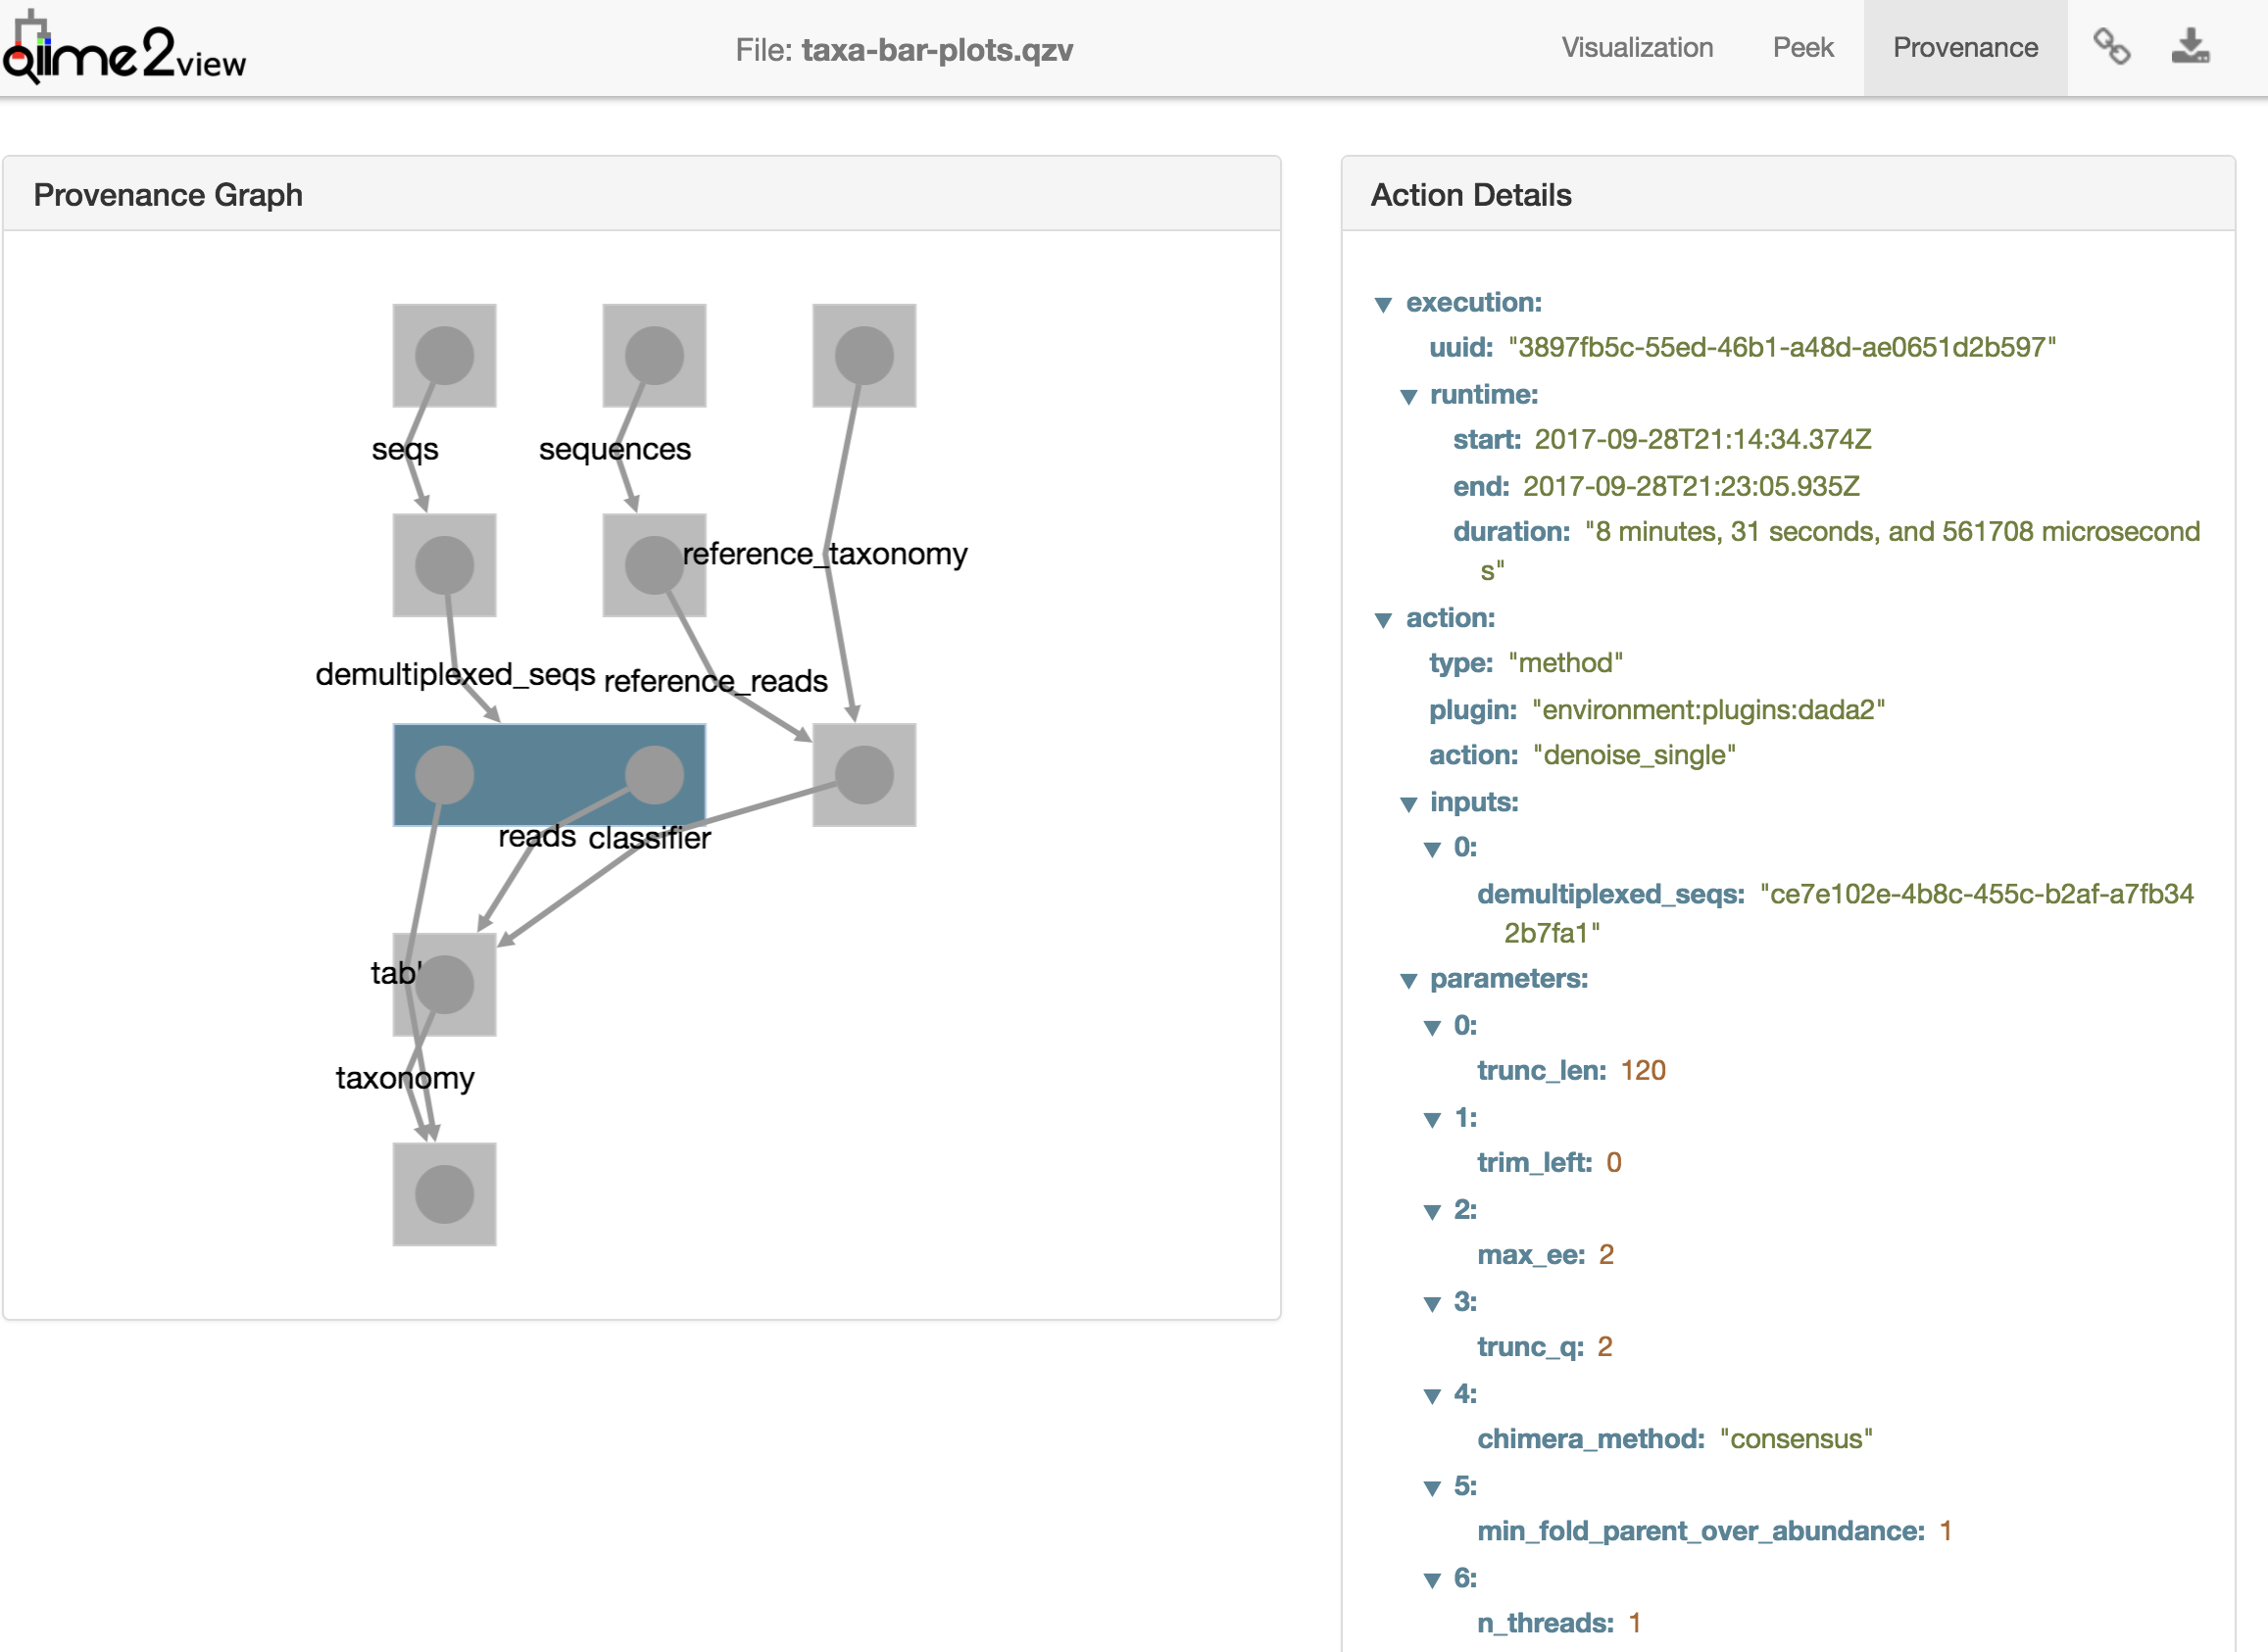
\includegraphics[width=\textwidth]{figures/provenance_graph.png}
\caption[Diagram of the history (provenance) of a QIIME 2 Artifact]%
{Diagram of the history (i.e. provenance) of a QIIME 2 Artifact. At left, a
directed, acyclic graph tracing this history from initial data import into QIIME
2, through the creation of a visualization for analytical interpretation or
publication, from top to bottom. Graph nodes represent QIIME 2 results, and
edges represent the actions performed to produce them. Graph nodes are composed
of one or more circles inside of a rectangle. The circles represent Results, and
the rectangles represent the actions that produced those results. (An Action may
produce one or more Results.) Graph edges describe the “movement” of Results
through an analysis; an edge originates in some Result, and “points at” any
Actions that used that result as an input. At right are the “action details”
captured during the creation of the two nodes highlighted in blue. QIIME 2
captures unique result identifiers, software version information, details on all
commands and parameters used, and computational resource use.}
\label{fig:provenance_graph}
\end{figure}

Khan et al [6] propose a framework of best practices for provenance capture,
many of which are satisfied by QIIME 2’s existing provenance capture system.
Data processing is done with versioned software rather than manual data
manipulation. All commands executed are recorded, along with their parameters,
and the versions of software they ran on. These software environments are
documented in provenance at run time, using the git version control system to
indicate modifications made to installed QIIME 2 packages. Basic information on
the hardware environment is recorded. Human-interpretable diagrams of result
history can be easily generated from any result and explored in a web browser
with no software installation needed. Result “archives” are formatted
consistently in clearly-defined ways, and when stored on disk they are packaged
in a common zip file format that is likely to be accessible across systems for
the foreseeable future.

The primary theoretical requirements for reproducing an in silico analysis in
QIIME 2 are met. However, the practical costs of doing so remain prohibitive.
Consider a relatively straightforward QIIME 2 analysis of a longitudinal data
set. We might import data from a single run of biological sequences generated by
a sequencing machine, and then analyze it, visualizing taxonomic composition,
alpha and beta diversity, changes in some important metrics over time, and
differential abundance between samples of interest. This analysis might require
25-30 discrete commands be run, producing 100 data outputs and figures. In order
to reproduce the analysis manually, the user would need to assemble each of
those commands from the serialized “action detail” data captured in provenance. 

In addition, the decentralized nature of QIIME 2’s provenance capture means that
history is captured on a per-result basis. There is no representation of a
complete workflow or analysis. In order to recreate a workflow, then, the user
must “re-assemble” a meaningful analysis from the provenance of many different
QIIME 2 results. This would require a clear understanding of what all of those
results are and what they mean in the context of the analysis, or a tremendous
and often redundant effort, reading the provenance of all 100 result objects and
knitting them together into runnable code for the 25-30 actions that produced
them. Even if we could assume user expertise sufficient to do the work
efficiently, the process would be painstaking and prone to human error. 

%%
%%
%%      4
%%
%%
\section{Reproducible research goals}

Breaking the expertise barrier described above has been a target of
computational reproducibility since at least Claerbout in 1992, whose team
published scientific work in digital media, and included in each figure’s
caption references and/or buttons that allowed trivial re-running of the
analysis that created that figure. They claimed that in this reproducible work,
“[j]udgement of the reproducibility of computationally oriented research no
longer requires an expert—a clerk can do it” (as cited in Plesser 2018, 76).
This “one-click” approach to reproducibility provides clear value for its
simplicity in corroborating the provenance of a single figure, and so is a
useful end goal to consider in the broader context of possible positive outcomes
from reproducible research.

Gunderson and Kjensmo, in their work on reproducibility in Artificial
Intelligence (AI), propose a hierarchical three-value system for ranking the
reproducibility of an AI based upon that AI’s degree of generality. 
\begin{itemize}
    \item Experiment Reproducible systems “produce the same results when [the same implementation is] executed on the same data."
    \item Data Reproducible systems produce the same results when executing “an alternative implementation of the AI method… on the same data.”
    \item Method Reproducible systems produce the same results when executing “an alternative implementation of the AI method… on different data”.[8]
\end{itemize}
% TODO: Inexplicably, the rest of the document indents if we don't end twice here.
\end{itemize}

The Turing Way Community’s definitions of “Reproducible”, “Robust”, and
“Generalisable” align (respectively) with these definitions, but exchange a
clear ordering for the ability to include an additional combination of factors,
defining:

\begin{itemize}
    \item “Replicable” systems “produce qualitatively similar answers”, when “the same analysis is performed on different datasets” \parencite{community_definitions_2021}.
\end{itemize}

Though varying slightly in scope and intent, these two systems both classify
distinct “types of reproducibility”, based on study design or outcome. There is
no “correct” or standard nomenclature in the literature, so we will impose a
Gunderson-like hierarchy on the Turing Way terminology here. (Figure \ref{fig:repro_classes})

\begin{figure}[htbp]
\centering
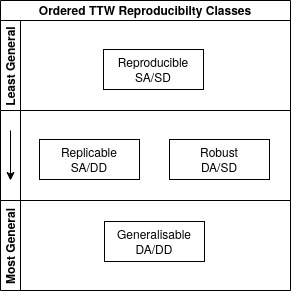
\includegraphics[width=.5\textwidth]{figures/repro_outcomes.jpg}
\caption[Hierarchically arranged reproducibility classes]%
{In this figure, Turing Way reproducibility classes are ordered in a
Gunderson-like hierarchy based on generality. Each class includes a pair of
descriptive two-letter codes, where the first letter abbreviates either Same or
Different, and the second letter Data or Analysis. For example, a Robust study
is coded DA/SD because it achieves the same results using a Different Analysis
of the Same Data.}
\label{fig:repro_classes}
\end{figure}

The value of Claerbout’s simple “one-click” approach breaks down once we
acknowledge that the fundamental goals of reproducibility often extend beyond
simple corroboration. As Shiffrin et al put it, "an effect valid in only one
exact context and not others is not usually useful and important. We want to
report effects that are reliable, important, are of scientific value, and
generalize to similar settings".[11] A one-click-reproducible figure achieves
only “reproducibility” - the lowest level of generality. It allows us to
corroborate that the software and the data produce a deterministic result, but
tells us nothing meaningful about the correctness of either. Investigating this
further would still require an expert to consider the data, read the source
code, and make their own judgment.

Replicable and robust studies provide a higher level of generality. “Robust
results show that the work is not dependent on the specificities of [e.g.] the
programming language chosen to perform the analysis”
\parencite{community_definitions_2021}, and replicable results
play a similar role in validating that the results are not just an artifact of
overfitting to the data. Generalisable results provide the highest possible
level of generality without necessarily providing generalized results. More work
may be required, but we can think of generalisable studies as the building
blocks of generalized scientific conclusions. Studies that are generalisable
likely meet the requirements for Goodman’s Inferential reproducibility.

With this framework in place, it becomes clear that there are many valuable
“reproducibility outcomes” that can grow from the foundation of Methods
Reproducibility. When researchers provide adequate “reproducibility
documentation”, we are able to corroborate studies, expand, and extend initial
work toward generalized conclusions. If the primary goal of scientific
reproducibility is to support the confirmation or questioning of the
truthfulness of scientific results, reproducibility tools should strive to
support all of these user stories:
\begin{itemize}
    \item Identification: a user can confirm that reproducibility documentation is directly relevant to some published result or results.
    \item Validation: a researcher or reviewer can confirm the integrity of their own or someone else’s results.
    \item Reproduction: a user can perform “simple” corroboration that the same data, compute system, and methods produce the same results.
    \item Extension/Generalization: a user can extend a reproducible analysis through changes in data, compute system, and/or analytical method without unreasonable operational costs.
    \item Scaling/Automation: reproducibility documentation should support extension to the scale of large meta-analysis.
\end{itemize}

In addition to these concrete outcomes, I propose that strong reproducibility
practices confer a number of critical “soft” benefits to science and its
practitioners. In an age of rapidly increasing information availability,
scientific specialization, and exponential growth in the available literature,
there are demonstrable costs to new researchers, and an increasing need for
collaboration in many fields.[11] Schiffrin et al argue that "current funding
levels and limited resources of time, equipment, and personnel ensure that
exploratory science cannot be conducted at a level of sophistication that
ensures complete reproducibility…. one must accept the inevitability of error
while doing what is possible to minimize it." Shiffrin’s core argument is that
science is a trial and error process with similarities to evolutionary
processes, and that rapid iteration (and frequent failure) have been and will
continue to be meaningful parts of the development of knowledge. Our goal, then,
can be framed in terms of “doing what is possible to minimize [the inevitability
of error]” by building tools that cost little to learn and use, and mitigate
important challenges, including many set out in the same paper: “The amount of
data being collected, the number of scientific journals… and scientific
information generally, has outstripped human ability to comprehend and act upon
those data,” and “increasing specialization may reduce progress by delaying the
age at which [younger scientists] can contribute."[11]

Shiffrin et al’s focus on reducing practical barriers to the conduct of
impactful science is important. Their suggestions that we prioritize new
exploratory and translational work, and prioritize study extension and
generalization over strict corroboration are reasonable compromises in the face
of limited research funding. In order to keep the practice of science
approachable and sustainable, we must also be willing to adopt direct remedies
to the reproducibility crisis that benefit both the conduct of science and the
utility of scientific results to practitioners. Software tools that actively
support comprehensive computational reproducibility documentation are a clear
candidate, with potential to reduce the risk of paper retraction, facilitate
collaboration and review, improve the continuity and impact of work, and
increase the efficiency of writing and publishing \parencite{community_added_2021},
with relatively low operational costs.

The potential benefits are enormous. Supporting public data access allows us to
wring the most possible value out of expensive data collection processes. With
sufficient effort and creativity, even highly protected private data can be
leveraged to provide ongoing public value without compromising its privacy.[28]
Strong reproducibility documentation practices provide a basis for complete
attribution, allowing us to appropriately credit prior researchers and method
developers for their contributions to the field. This, in turn, helps
incentivize and support the development and maintenance of
critical-but-invisible methodological and software tools. And as we leave
Claerebout’s one-click figure corroborator behind for more accessible tools for
reporting and interacting with study methods, we open the door to solving the
key problems that contemporary researchers face - reducing the practical and
intellectual costs of supporting and enacting scientific reproducibility.

These two facets of reproducibility - documentation and enaction - are
inseparable. If no one ever undertook to reproduce scientific work, there would
be no value in documenting (in the broadest sense) for reproduction. Without
adequate documentation (again in the broadest sense), it is impossible to
undertake the reproduction or extension of any study. Any solution that proposes
to improve reproducibility must satisfy users from both groups. It should a)
simplify the process of documenting the production of a scientific result, and
b) simplify the process of reproducing and extending that result. We should
“make reproducible research too easy not to do.”[12] Claerbout’s early work, by
leaning on automation, sets a high standard for ease of use, but may fail to
address the expertise problem in cases where simple corroboration is inadequate.

Biologists today have widely varying levels of biological and computational
expertise. They work in the field, in wet labs, in computational settings, and
in software roles. They collaborate across research domains. They use
spreadsheets, R and Python, matlab, stata, C, C++, FORTRAN, and many other
programming languages. They interact with data through command line interfaces
(CLIs), application programming interfaces (APIs), Graphical User Interfaces
(GUIs), with self-documenting notebooks (e.g. Jupyter Notebook, RMarkdown),
through workflow description languages (e.g. CWL, WDL, NextFlow), and so on ad
infinitum. It is unreasonable to expect any one researcher to have fluency with
all of these tools. It would be counterproductive to make the enactment of
reproducibility heavily dependent on any of them.

If we are to overcome the perception that “the remedies proposed to deal with
the reproducibility crisis will inevitably increase the research overhead”[11],
reproducibility solutions must be easy to use, and must help us to solve
meaningful problems. They should help us to digest highly technical information
as quickly as possible. They should minimize the technical overhead to
understanding study methods well enough to apply, modify, or extend them. They
should help us communicate our methods and results to collaborators with
different skill sets.

In order to effectively support scientific reproducibility today, tools should
aim for:
\begin{itemize}
    \item Completeness: tools for reproducibility should attempt to fully support study reproduction.
    \item Ease of documentation: research should self-document to the greatest extent possible.
    \item Ease of reproduction: Enacting reproduction should be as easy as possible.
    \item Ease of automation: parseable, executable, and/or executed outputs should be supported.
    \item Readability: research documentation should be readable by human users.
    \item Learning-ready: research documentation should support learning with the minimum possible requirement of specialized expertise.
    \item Interpretation and Communication: research documentation should support readability and sharing across technical barriers like programming languages or user interfaces.
\end{itemize}


%%
%%
%%      5
%%
%%
\section{QIIME 2 concepts}

In this section, I will discuss features of the QIIME 2 Framework and associated
tools that are relevant to the implementation of the reproducibility goals
stated above. 

The QIIME 2 team has attempted to reduce confusion around frequently-used (and
frequently overloaded) terminology by explicitly defining and documenting key
terms for users and developers in the context of the software platform.[5] We
will rely on some of these definitions heavily, and will discuss them here
alongside other key features. These QIIME 2-specific terms will be capitalized
whenever possible to reduce confusion with other definitions.

\subsection{The QIIME 2 Framework (the Framework)}
The QIIME 2 framework is an “engine of orchestration that enables QIIME 2 to
function together as a cohesive unit.”[5] The framework is both interface
agnostic and domain agnostic, but implements the common core of functionality
that allows users to interact with bioinformatics methods (defined in plugins)
through a variety of different interfaces. This includes key features like a
Semantic Type system that enforces type validity and supports pipelining and
cross-plugin interoperability, and systems for retrospective provenance capture
and the construction of consistently structured Archives.

QIIME 2 plugins declare their available methods (and other key concepts) to the
Framework using a “registration” API. Registered plugins can be used by any
QIIME 2 interface. This provides significant flexibility for users, and added
value for plugin developers, who get API, CLI, GUI, and workflow language (WL)
interfaces “free” through the framework.

\subsection{QIIME 2 Actions}
Defined in the documentation as “a generic term to describe a concrete Method,
Visualizer, or Pipeline, Actions accept parameters and/or files (Artifacts or
Metadata) as input, and generate some kind of output.” Users of QIIME 2 interact
with their data primarily through the use of these plugin-defined Actions. Some
Actions (specifically Pipelines) operate by executing multiple other actions.

\subsection{QIIME 2 Results}
Defined in the documentation as “a general term for an Artifact or a
Visualization,” Results are the primary type of output produced by QIIME 2, and
can be differentiated in terms of intended use. Artifacts are intermediate data
results intended to be read by QIIME 2 itself. Visualizations are terminal
outputs, intended to be read and interacted with by humans. 

For example, an Artifact of the FeatureTable semantic type, stored on disk as a
.qza file, contains binary-encoded data which would be very difficult for a
human user to interpret, but which provides an efficient computer-readable
format. A Visualization might be made from the Artifact by passing it into a
Visualizer Action.

Actions produce one or many Results as outputs.

\subsection{Archive Versions}
The documentation defines an Archive as “the directory structure of a QIIME 2
Result”, containing “at least a root directory (named by UUID) and a VERSION
file within that directory.” 

Archives are formally defined and registered in the QIIME 2 archiver code, and
any change to the structure of a QIIME 2 archive must be implemented as a new
archive version. As QIIME 2 has grown in capability and complexity, six
backwards-compatible archive versions have been registered. Any reproducibility
tool aiming to support all QIIME 2 Results must account for variation in Archive
Versions.

The first (v0) Archive Version did not include any provenance data, because
QIIME 2 did not capture provenance at that early stage in its development.
Subsequent versions capture provenance data in a provenance directory within the
Archive’s root directory.

\subsection{UUIDs}
Both QIIME 2 and the Provenance Replay tools described here make frequent use of
v4 (random) UUIDs.[13] (We will refer to these simply as UUIDs going forward.)
These are randomly-generated 128-bit labels composed of 32 hexadecimal
characters broken by hyphens into character groups with lengths of 8-4-4-4-12
characters each. These identifiers have no special significance, but rather were
selected for use because they are a common and convenient way to label uniquely.
Though collisions are theoretically possible, the 5.3×1036 possible v4 UUIDs
make the probability of collision vanishingly small in the contexts where we
apply them.

The QIIME 2 framework assigns every Result a UUID, providing a valuable property
for checking and tracking Result identity. 

\subsection{MD5 Checksums}
Beginning with Archive Version 5 (released in QIIME 2 2018.11), Archives contain an md5sum-formatted[14, 15] checksums.md5 file in their root directory. This is a digest of (checksum, relative file path) pairs, where each checksum is a hash of the file contents. Any change to the file contents is highly probable to result in a change to the file’s hash. The MD5Sum algorithm is cryptographically broken, but still widely used in non-secure contexts. Barring malicious tampering, checksums allow us to confirm the integrity of the contents of any QIIME 2 Archive.

\subsection{Archive and Provenance data structure}
The goals, structure, and contents of QIIME 2 Archives are treated at length in
the “How Data is Stored” section of the developer documentation[35]. A few key
ideas are worth mentioning here.

\begin{itemize}
    \item The QIIME 2 Archiver currently stores Archives to disk as ZIP files[16, 17], because ZIP is a ubiquitous, compact, open, and well understood archive file format.
    \item Other ArchiveFormats may exist in the future.
    \item Data and provenance are stored separately, allowing provenance data formats to be centrally defined, while allowing plugins to define their own preferred data structure. We need not concern ourselves with the contents of the data directory here.
    \item The provenance directory of an Archive (if present) contains the provenance data for the Result whose data is stored in the archive, alongside a non-hierarchically-organized artifacts directory containing provenance data for all of the results required to create that Result - its dependencies, or ancestors. Study data is not stored in this archive for these ancestor Results - only provenance information. We may refer to the Result whose data is stored in an archive as the “terminal”, or “root” Result or node for the Archive.
    \item Each ancestor Result’s provenance data is stored in a directory named with that Result’s UUID.
    \item QIIME 2 Results are portable across versions of QIIME 2. As a result, an Archive may contain provenance data conforming to an arbitrary number of Archive Format Version specifications.
\end{itemize}

\subsection{QIIME 2 release/packaging model}
At the time of writing, the QIIME 2 Framework is packaged with many “core”
plugins on a quarterly release cycle. Most users install a conda package,
container, or virtual machine, and get access to commonly used plugins.
Third-party plugins must be installed separately, however, and there is no
guarantee that a plugin used in a prior analysis will be present in a user’s
current QIIME 2 deployment.

This release model is currently in transition towards a less centralized and
potentially less consistent model, in which third-party plugins are likely to
play a more significant role. Awareness of this dynamic is likely to be
important to any reproducibility tool targeting QIIME 2.

\subsection{Potential users of Provenance Replay tools}
So far, we have focused primarily on the case that human researchers can derive
value from tools for in silico reproducibility. It is important to note that the
consumers of these tools may be human or machine “users”. Study goals vary, as
do software requirements, and a strong case can be made for the value of
reproducibility tools that allow for the large-scale, mechanized corroboration
or extension of existing Results.

For example, the Knight Lab team at UCSD is interested in using provenance
replay within their QIITA software platform, allowing them to identify
performance bottlenecks in QIIME 2 workflows. Users' QIIME 2 analyses could be
replayed and profiled for performance bottlenecks, supporting targeted
development of performance optimizations.[46]

Full, “touchless” automation of reproducibility solutions, especially in the
contexts of corroboration and meta-analysis, is a valuable long-term target, so
it is worth noting that machine users may have a different set of priorities
than human users of the software. Automated systems are more likely to need high
levels of time and space efficiency when working with large data. These are
goals I have attempted to support directly through development, and by tracking
clear opportunities for improvement in a public issue tracker[47, Issues #29,
60, 62].

Automation also requires a level of determinism adequate to alleviate the need
for human judgment. The current implementation of Provenance Replay, for reasons
that will be discussed below, is unable to support the full automation of study
reproduction. Changes have been proposed to the QIIME 2 Framework that may allow
this work to move forward in the near future. At the time of writing, however,
human users are our primary target.


\section{Provenance Replay for QIIME 2}

The work presented here attempts to improve computational methods
reproducibility in QIIME 2 by reducing the practical overhead of important
reproducibility outcomes. Built around the automated, decentralized provenance
capture implemented in the QIIME 2 Framework, I present user-friendly tools to
validate the integrity of QIIME 2 Results, parse the provenance data they
contain, and programmatically generate executable scripts that allow for the
reproduction, study, and extension of the source analysis.

The software, written in Python 3.8, depends heavily on the Python standard
library, NetworkX[18], pyyaml[19], and QIIME 2 itself, from which it takes
advantage especially of the PluginManager and the Usage API. Called “Provenance
Replay”, the software ingests QIIME 2 Results and parses their provenance data
into a Directed Acyclic Graph (DAG) implemented as a NetworkX DiGraph. It
produces outputs by subsetting and manipulating this DiGraph and its contents.
Outputs include bibtex-formatted[20] citations for all Actions used in a
computational analysis, and executable scripts targeting the user’s preferred
QIIME 2 interface. Users interact with the software through a command-line
interface implemented with Click[20], or with a Python3 API. A graphical user
interface built on the Galaxy platform[21] is targeted for future development.
                     %<Insert your chapters here; I recommend to use
%%%%%%%%%%%%%%%%%%%%%%%%%%%%%%%%%%%
% Chapter 2 
%%%%%%%%%%%%%%%%%%%%%%%%%%%%%%%%%%
\chapter{Provenance Replay Software}
The Provenance Replay software, as implemented, attempts to meet the loose
requirements funded by the US National Cancer Institute’s Informatics Technology
for Cancer Research program (grant number 1U24CA248454-01). In addition, we
undertook an internal requirements engineering process, involving requirements
elicitation by focus group, and requirements validation using Technology
Acceptance Model (TAM)[29] and Net Promoter Score[30] (NPS)-based survey
instruments. These two processes (initial development and requirements
engineering research) will be discussed in separate sections roughly
corresponding to the chronological order of the work, in which an Alpha release
version of Provenance Replay was developed first based on funding agency
requirements and literature review, and requirements engineering processes were
used to refine software requirements and validate the success of the initial
implementation. 

%%
%%
%%      1
%%
%%
\section{Overview}

As initially proposed, the aim of Provenance Replay is to “generate executable
code directly from a Result’s provenance”[46]. Framed as functional
requirements:
\begin{itemize}
    \item Provenance Replay must ingest QIIME 2 Results, and from them produce command-line (BASH) and Python scripts
    \item These scripts must be usable with QIIME 2’s q2cli and Python 3 API interfaces
\end{itemize}

% EXAMPLE: don't indent "new paragraph" after itemize bullet list
\noindent Framed as a user story: \\
A QIIME 2 user, in a setting where new data must continuously be
merged with existing data, wants to parse a result from the previous iteration
of an analysis and use the resulting script to produce the same result after
incorporating the new data. 

I developed a Python package, \texttt{provenance\_lib}, to meet these basic
requirements.  The modular design targets two primary processes - the parsing of
provenance data from QIIME 2 Results, and “replay” tools which output executable
scripts, along with other reproducibility documentation designed to address the
challenges discussed above. These outputs are self-documenting, and leverage
UUIDs to make them identifiable as products of specific QIIME 2 Results. A third
module implements MD5 checksum-based validation of archive provenance, capable
of alerting a user to losses of integrity in their Results. 

This functionality was developed with human users as the primary constituency,
and implements both a Python 3 API and a command line interface. Reproducibility
scripts can be produced targeting the corresponding QIIME 2 Python 3 API and the
q2cli command line interface, allowing users to produce and consume Provenance
Replay outputs with their preferred interface. Though not the primary target,
design choices that support scaling and automation have been made where
possible, and replay commands offer many parameters to enable replay actions to
be faster and more resilient to compromises in data quality.

The following subsections explore the high-level architecture and select design
decisions made in the creation of this software.

%%
%%
%%      2
%%
%%
\section{Parsing provenance data from Archives}

The components of QIIME 2 Archives required for provenance parsing (e.g. the
VERSION files and the contents of the provenance directory) are consistently
formatted, with variations clearly defined and versioned in the QIIME 2 core
codebase. QIIME 2 guarantees that all Archives will contain a root directory
named with the archive UUID - this serves as the Archive’s identity, and I will
refer to it when needed as the “root UUID”. Within this root directory, all
archives contain a VERSION file, which holds the necessary information to
identify what version of the Archive Format specification this archive complies
with.[31] By determining which archive version we are working with, it is
possible to identify and parse all files within the Archive which are relevant
to Provenance Replay.

We will discuss the handling of various archive versions in greater detail
below. Here we will focus on the lower-level work of parsing the relevant data
from a version-5 Archive, the current and most complex Archive Format version.
(Figure \ref{fig:archive_structure})

\begin{figure}[htbp]
\centering
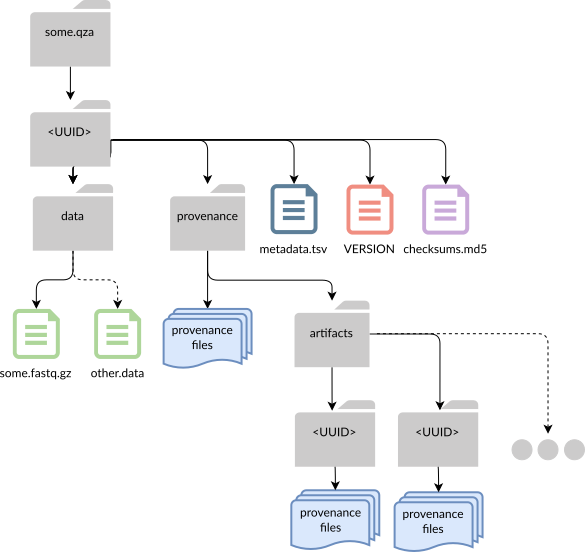
\includegraphics[width=\textwidth]{figures/archive_structure.png}
\caption[Diagram of the structure of a version-5 QIIME 2 Archive]%
{A graphical representation of the structure of a version 5 QIIME 2 Archive
stored as a Zip Archive. The directory structure is represented by gray
directory icons, with arrows indicating levels of nesting, wherein the parent
directory “points to” all of its contents. Single files are represented by the
“folded-corner” file icons, and a “file collection” icon in blue represents the
collection of files that contain provenance data. This is shown in an expanded
view in the following figure.}
\label{fig:archive_structure}
\end{figure}
A Result stored on disk as a zip file may have any filesystem-compliant
filename, and will be suffixed with .qza or .qzv by default. Internally, the
root directory is named with the UUID representing the Results stored within the
data directory. In a Version 5 Archive, the root directory contains an MD5sum
digest, a VERSION file detailing the Archive version and the version of the
QIIME 2 Framework that produced the Result, and a metadata.yaml file describing
primary characteristics of the Result itself. The data directory holds the
Result data, and the provenance directory contains captured provenance data.
Note that the artifacts directory may contain an arbitrary number of
provenance-files directories, and that these contain only provenance
information. By not capturing ancestral data in provenance, we reduce the risk
of unmanageably-sized Archives, at the “cost” of users needing multiple archives
to hold all of the data from a given analysis. Users generally manage this
complexity by organizing their Results in a file system, though more
sophisticated solutions are possible (e.g. a database mapping UUIDs to resource
IDs or locations on disk). (Figure \ref{fig:provenance_files})

\begin{figure}[htp]
\centering
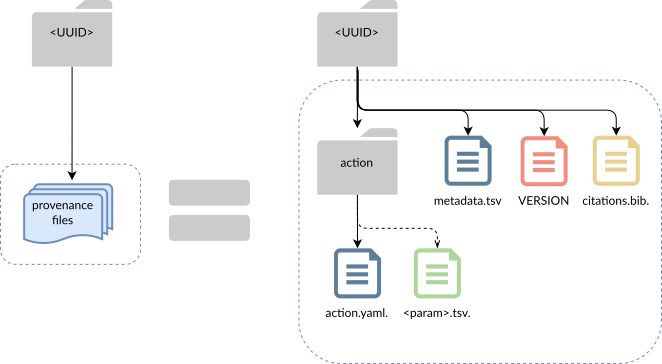
\includegraphics[width=\textwidth]{figures/prov_files.png}
\caption[Diagram of the provenance file directories in a QIIME 2 Archive]%
{An expanded graphical representation of the contents of a directory of
provenance files from a version 5 Archive. Each of these directories is uniquely
identified with the UUID of the ancestor result whose provenance is described
within. Information about the action that produced this Result is stored in an
action directory, including .tsv-formatted files representing any metadata used
in that action. Every provenance directory contains its own VERSION file,
metadata.yaml, and a bibtex-formatted list of relevant citations.}
\label{fig:provenance_files}
\end{figure}
VERSION files are specified in a simple, custom format. The root-level VERSION
file is checked for validity against a regular expression. If valid, the Archive
version is parsed using Python’s standard-library string manipulation methods,
and used to determine how to parse the rest of the archive. Bibtex files are
parsed with the bibtexparser library[20], pandas[32, 33] is used to read the
metadata .tsv files, and pyyaml is used to handle the critical metadata.yaml and
action.yaml files.

A number of custom-defined constructors are required in order to parse these
YAML files, as pyyaml does not by default support serializing and deserializing
Python sets, or the QIIME 2-specific !cite, !color, !metadata, !no-provenance,
and !ref tags. The safe\_loader is used for all deserialization to reduce the
risk of malicious code injection.

Parsed provenance information for each Result is captured in a ProvNode object.
These serve as the data payloads in our provenance DAG. The ProvNode class is
implemented with a highly flexible initialization method, which initializes
component classes if the files they depend on are provided. ProvNode attributes
which depend on these component classes are frequently implemented using
Python’s @property decorator to allow for the possibility of absence, and the
ProvNode itself always has a property has\_provenance which downstream code can
use as a guard against nodes with no provenance data at all. In this way,
ProvNodes can be parsed from Results that have Archive Format versions with
varying levels of complexity. 

\begin{figure}[htp]
\centering
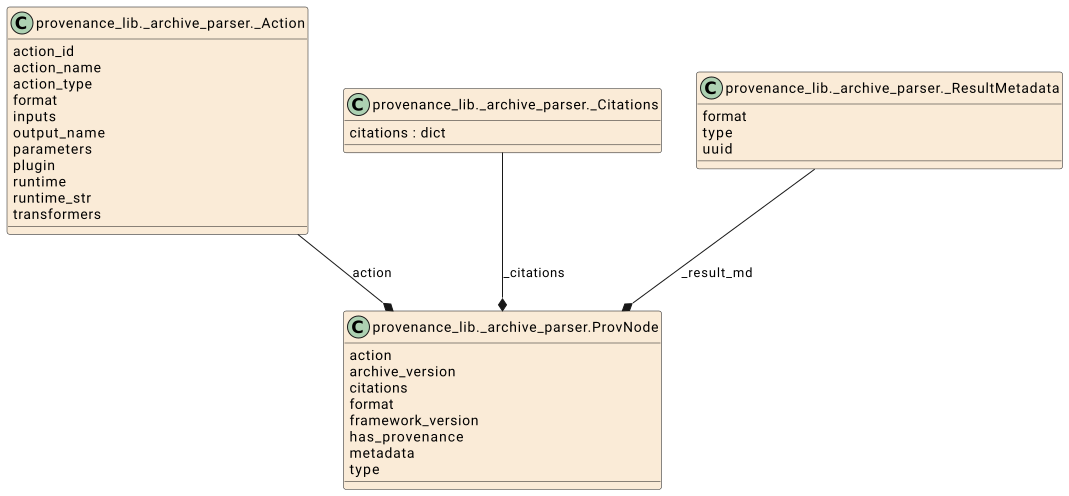
\includegraphics[width=\textwidth]{figures/ProvNode_UML.png}
\caption[UML Class diagram of the ProvNode class and its components]%
{A UML class diagram of the ProvNode class and its component classes, each of
which represents one of the key provenance files - action.yaml, citations.bib,
and metadata.yaml.}
\label{fig:ProvNode_UML}
\end{figure}

%%
%%
%%      3
%%
%%
\section{Cross-version analyses and handling no-provenance nodes}

The provenance parser attempts to represent provenance as completely as possible
given the available data. All known nodes are represented, regardless of whether
we have provenance data for them. Nodes without provenance data may exist, and
this impacts the construction of DAGs in some important ways.

If a V1+ archive was constructed to represent a Result R with at least one V0
Result (S) as an ancestor, then for some subgraph of the DAG representing R,
there is no provenance data to parse describing S. To be more specific, there
will be no provenance directory named with S’s UUID saved in R’s
provenance/artifacts directory. A record of S’s UUID will, however, be saved in
the action.yaml file of S’s immediate descendant.

DiGraph nodes are literally UUID strings. The minimal DiGraph node has the
following attributes:
\begin{itemize}
    \item has\_provenance - a flag indicating whether provenance data exists for this node
    \item node\_data - either a ProvNode payload, or None
\end{itemize}

The provenance parser, for completeness, must include a minimal node in the
DiGraph constructed to represent R during initial parsing. For safety in working
with these graphs, archive parsers first construct ProvNode payloads for nodes
which have provenance, add any no-provenance nodes to the graph, and then check
each node for the absence of a provenance payload, setting the required
attributes in cases where they are missing. Consumer functions may safely
(without KeyError) check whether a node has\_provenance, and access ProvNode
properties appropriately if provenance exists.

%%
%%
%%      4
%%
%%
\section{Provenance Parsers and Dispatch for provenance parsing}

Provenance Replay implements an extensible dispatch system for parsing
provenance. All parsing is done by implementations of an abstract base class
Parser, which defines the basic contract for any provenance parser. 
\begin{itemize}
    \item A Parser implements the classmethod get\_parse, which ingests arbitrary input data. It either returns a Parser that can parse that data, or it raises an Error.
    \item A Parser implements the method parse\_prov, which ingests an appropriate data payload, parses it, and returns a ParserResults object.
    \item A Parser has a string attribute accepted\_data\_types required for the production of error messages when the parser receives a type of data it cannot parse.
\end{itemize}

Parsers that meet this contract may be registered in parse.select\_parser.
Briefly, parsing proceeds as follows. A user calls the ProvDAG class, which is a
domain-specific wrapper around a networkx.DiGraph, with some input data.
ProvDAG.\_\_init\_\_ uses the parse\_provenance function, which calls
parse.select\_parser with the input data. This function iterates over the known
parsers, testing the data payload against their get\_parser methods and
aggregating the errors that result. 

If a Parser that can parse the payload is found, that parser will be returned
immediately, and aggregated errors will not be reported. The returned Parser
instance’s parse\_prov method parses the input data payload and returns a
ParserResults object. A ProvDAG is then initialized from the DiGraph and other
data contained in the ParserResult, exposing user-facing methods for accessing
and manipulating the aggregated provenance data.

ParserResults objects function as a common data interface between the Parsers
which create them, and the ProvDAG class. (Figure \ref{fig:ParserResultsUML})

\begin{figure}[htp]
\centering
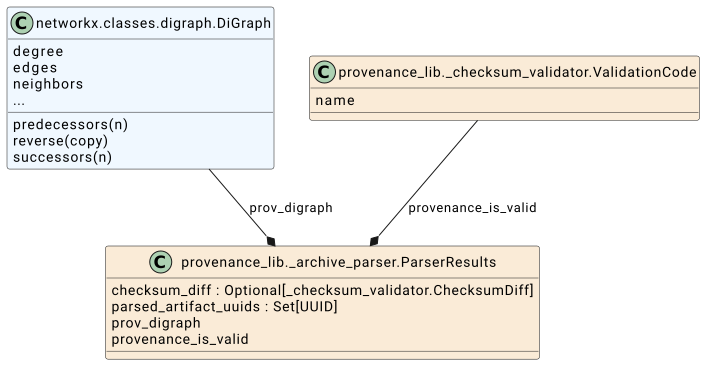
\includegraphics[width=\textwidth]{figures/ParserResultsUML.png}
\caption[UML Class diagram of the ParserResults class and its components]%
{A UML class diagram of the ParserResults object with associated properties.
Classes in beige are locally defined, while classes in blue are imported from
NetworkX.}
\label{fig:ParserResultsUML}
\end{figure}

If no adequate Parser is found, an UnparseableDataError is raised, and the user
receives a digest of error outputs which they can use to troubleshoot their
input data. Should external tools make use of provenance parsing, this custom
error type may simplify graceful error handling in cases where it is more
important to continue processing input data than to consider/correct failed
input data. 

Four “top-level” Parser implementations currently handle all parsing needs.
These are:
\begin{itemize}
    \item ProvDAGParser: parses a ProvDAG object, enabling the copying of ProvDAG objects
    \item EmptyParser: parses None enables the creation of empty ProvDAG objects
    \item ArchiveParser: parses a single QIIME 2 Archive
    \item DirectoryParser: parses a directory of QIIME2 Archives, returning a single ParserResults object which represents all parsed Archives in a single DiGraph
\end{itemize}

Parsers are responsible for deciding whether they can parse a data payload, and
are not required to return an instance of their own class. This flexibility
allows for the extension of individual Parsers to handle an arbitrary number of
related data types. For example, if ArchiveParser.get\_parse() receives any type
or version of QIIME 2 Archive, it will handle dispatch internally, returning an
instance of a child class of ArchiveParser designed to address the specific
needs of that type or version of Archive.

This architecture reduces coupling between the high-level parse\_provenance
function (and its callers), and the low-level parsing code, by replacing direct
dependencies with dependencies on a shared abstraction (Parser). Modifications
to existing Parsers are immaterial to the high-level code, and extending the
codebase with an additional “top-level” Parser requires only the implementation
and registration of the Parser. 

\begin{figure}[htp]
\centering
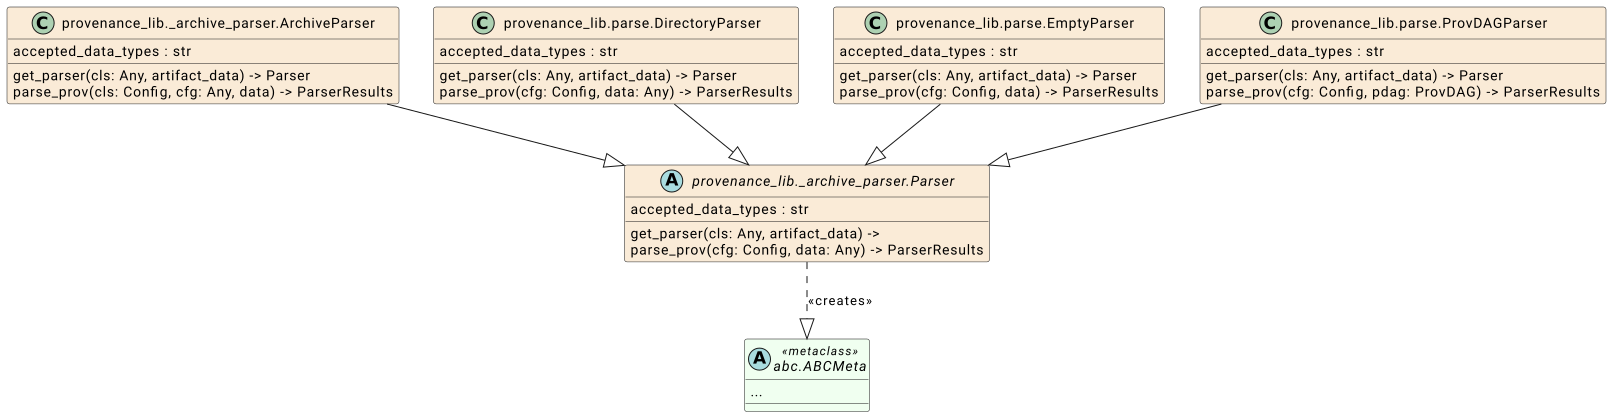
\includegraphics[width=\textwidth]{figures/allParsersUML.png}
\caption[UML Class diagram of the abstract Parser class and its implementations]%
{This UML class diagram describes the abstract Parser class and its top-level
implementations. The element notation “C” to the left of the class name
indicates a class, while “A” indicates an abstract class. Classes in beige are
locally defined, while classes in light green are imported from the standard
library. Note that many additional, specialized Parser implementations are
accessible through e.g. ArchiveParser.get\_parser.}
\label{fig:allParsersUML}
\end{figure}

%%
%%
%%      5
%%
%%
\section{Handling Changes in Archive structure over time}

The QIIME 2 Framework defines six Archive Format versions, numbered from 0 to 5,
which have increased in complexity as provenance capture has become more robust.
Results created in the earliest of these Archive Formats (v0) do not contain
provenance data at all. I have covered the details of these archive structure
changes at length in the developer documentation [34], so will focus on the
architectural decisions made to support this structure in Provenance Replay.
Archive Formats are explicitly versioned, because change is anticipated and must
be supported, so extensibility is a key non-functional requirement. 

Archive parsing proceeds roughly as follows.
\begin{enumerate}
    \item The parser uses filename data stored in its class attributes to identify all file paths present that should be parsed. These are grouped by Result.
    \item If any expected files are missing, the parser responds appropriately (e.g. raise/warn).
    \item The parser instantiates a ProvNode object for each Result by calling ProvNode with a collection of Result-specific filepaths.
    \begin{enumerate}
        \item[3.1.]ProvNode.\_\_init\_\_ iterates over whatever filepaths it receives, dispatching the actual parsing to appropriate helper functions. 
    \end{enumerate}
    \item The parser builds a DiGraph representing the provenance history of the Archive
    \item The parser returns a ParserResults containing this DiGraph and other attributes
\end{enumerate}

This approach forefronts extensibility through flexibility and encapsulation.
The ProvNode initializer is a generalist with no knowledge of the requirements
of the Parsers. Its single responsibility is to instantiate ProvNodes from the
data it receives, and it doesn’t need to know anything about archive versions -
only where to dispatch different files for parsing. If it gets the file, it
parses it. Parsers, on the other hand, are format-specific, and are responsible
for checking the integrity of their input data against their understanding of
the Archive Format version they target, collecting files and sending them out
for parsing, and returning the resulting ParserResults object.

To date, changes to Archive formats have generally been additive, and have
accreted in relatively small increments, which as a general trend lends itself
well to inheritance. In order to support a new Archive Format (v6) that captured
a new type of provenance file with every Result, we might only need to:
\begin{itemize}
    \item Define a class or function capable of the low-level parsing (e.g. loading serialized data)
    \item Add a check for the new file to ProvNode.\_\_init\_\_(), calling this class/function
    \item Subclass Parserv5, adding the new filename to the expected\_files\_in\_all\_nodes class attribute
\end{itemize}

% EXAMPLE: Caption to the right side of Figure
\begin{figure}[htp]
    \begin{minipage}[c]{0.5\textwidth}
        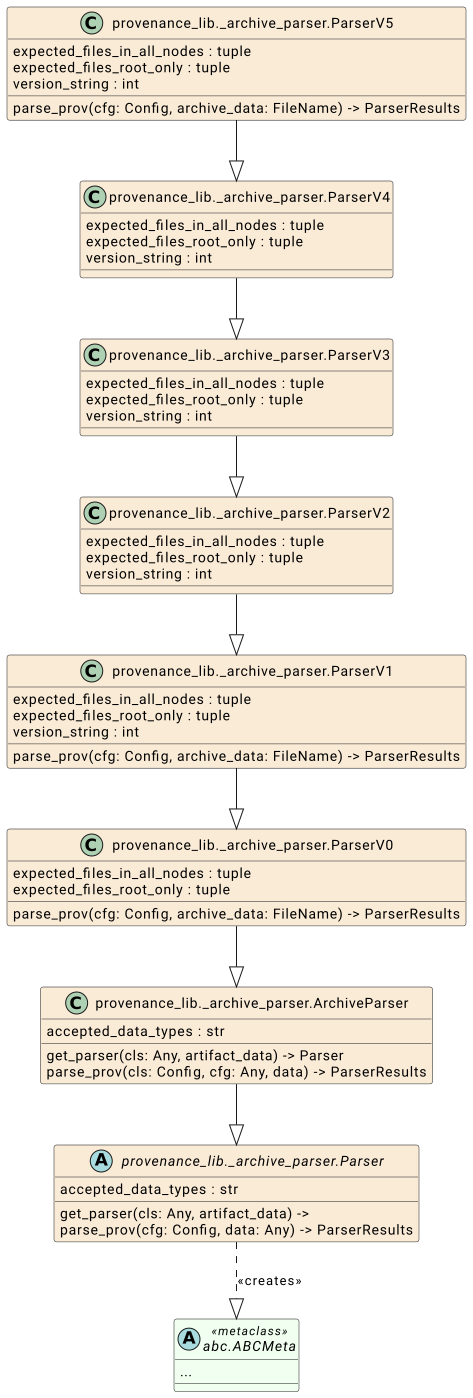
\includegraphics[width=\textwidth]{figures/archiveParserUML.png}
    \end{minipage}\hfill
    \begin{minipage}[c]{0.45\textwidth}
\caption[UML Class diagram of the Version-specific Archive Parsers]%
{This UML diagram depicts select features of the \_archive\_parser module. Classes
in beige are locally defined, while classes in light green are imported from the
standard library. The element notation “C” to the left of the class name
indicates a class, while “A” indicates an abstract class. The inheritance
structure used in the definition of version-specific archive parsers mirrors the
archive format definition itself in the QIIME 2 Framework, and dramatically
reduces the amount of redundant code, resulting in a smaller maintenance surface
area. Note that the get\_parser implementation in the ArchiveParser class can
return instances of any of the child parser implementations, and the parse\_prov
implementation in Parserv1 is used by all of the classes that depend on it.
Changes in parser behavior from V1-V5 are effected through simple changes in
class data, and ‘private’ helper methods like \_validate\_checksums}
    \end{minipage}
    % \label{fig:allParsersUML}
\end{figure}

Low-level parsing/loading work is handled by file-type-specific classes, which
load some type of data, and expose key values or behaviors as object properties
or methods. Strict validation of file contents is not performed (though it would
certainly be possible to do so). With the exception of a few key characteristics
(UUID, archive version number, etc.), the contents of these files are important
to the end user, but not to the Provenance Replay tool itself. By parsing and
providing all contents without, for example, schema validation, we can meet end
user needs with simpler and therefore more performant code.

This implementation allows some classes of extension to be made primarily by
manipulating class attributes, resulting in a minimal maintenance surface area.
Changes made to the structure of the action.yaml file in versions 2, 3 and 4
required no changes to the parser logic. The addition of a citations.bib file to
all Results in version 4 proceeded as described above. The addition of a
checksums.md5 file in the root directory for V5 required this process, plus the
re-implementation of a helper function, and a call to super().parse\_prov. The
code for all of these Parsers is minimal, as nearly all behavior is inherited. 
(Figure \ref{fig:parserCodeBlock})

% TODO: This ref ^ is borked, pointing to the prior figure

\begin{figure}[htp]
\centering
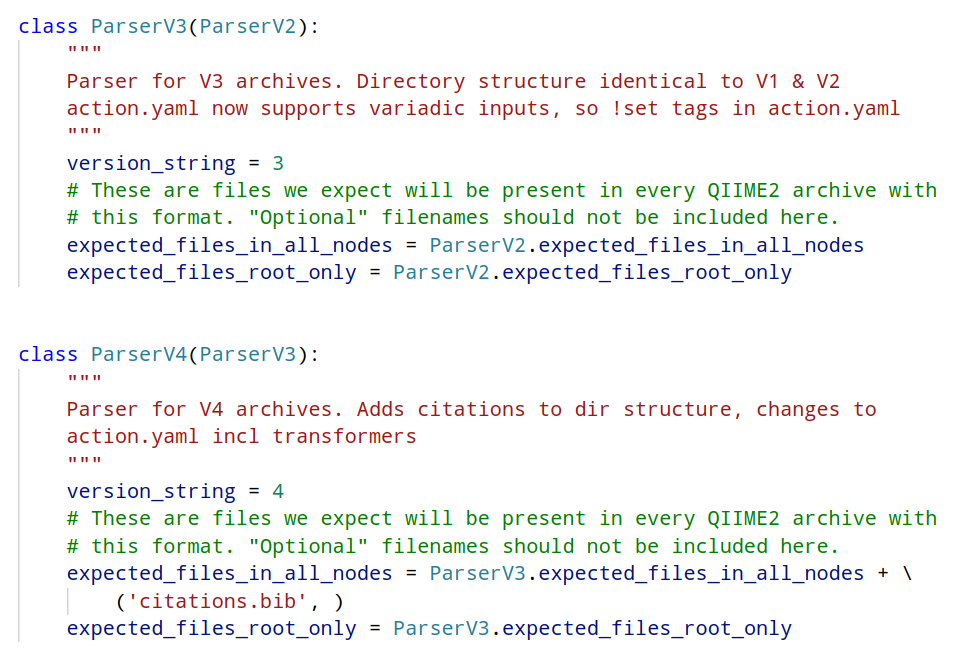
\includegraphics[width=\textwidth]{figures/parserCodeBlock.png}
\caption[Code snippet illustrating the value of inheritance to ArchiveParser Versions]%
{full code of the ParserV3 and ParserV4 classes, illustrating the value of
inheritance and low-level parser flexibility in reducing code surface area.}
\label{fig:parserCodeBlock}
\end{figure}

%%
%%
%%      6
%%
%%
\section{Representing single Results or full analyses with DiGraphs}

Many studies require information from more than one QIIME 2 Result in order to
adequately address their research questions. We must therefore support user
stories in which a user replays multiple Results into a single “analysis-level”
script. Failure to do so would result in users generating multiple replay
scripts with potentially high levels of duplication, and then manually or with
their own software tools, a) incurring unnecessary computing costs to generate
and then delete many duplicate Results, or b) incurring unnecessary researcher
or developer costs to merge these replay scripts for a single run without
duplicate Results. Either of these would likely be prone to user error. 

The provenance of a single QIIME 2 Result conforms to the properties of a
directed acyclic graph (DAG), with one or more “input” nodes and a single
terminal node representing the “root” node whose data is contained in the
Archive. Each node in the graph represents a Result, and each edge u → v
represents an action that took node u as an input and produced node v as an
output. A node can only be the product of one Action, so multiple in-edges to a
single node will always represent the same Action. We capture Action-specific
data in the graph nodes produced by that action, for loose parity with the
representation of that data in both the Archive structure and in the widely used
q2view provenance graph visualization. 

These DAGs are implemented as DiGraph objects, defined by the NetworkX library
for graph analysis. NetworkX was selected for many reasons. It is widely-used
and well-supported, offers most common graph operations built in, and supports
export to common graph visualization libraries (e.g. Cytoscape). There are a
number of significantly more performant graph libraries available for Python,
but as a pure Python library NetworkX presents a reduced risk of dependency
management challenges.

In our implementation, DiGraph nodes are literal UUID strings, with provenance
information stored as node attributes. NetworkX supports the creation of graphs
with user-defined hashable objects as nodes, but our approach results in a graph
in which common interactions with nodes (e.g. querying the graph, asserting
against node properties) are simpler and more intuitive.

QIIME 2 provenance data folders are archived in a non-hierarchical format for
reasons of simplicity and ease of access. Every parent Result’s provenance is
stored in its own UUID-named directory, and these are all placed into a single
parent directory. Creating a DiGraph, then, requires us to parse the provenance
data in each of these provenance directories, capturing ancestry information
about each node, and using it to define the edges that connect a node to its
input dependencies.

QIIME 2 Results are stored in independent Archives, and each archive contains
only the provenance data directly relevant to its own creation. It is common for
two Results from a single analysis to share many, or even all of their data
dependencies. DAGs with multiple terminal nodes are common, making the DAG a
natural fit for representing complete QIIME 2 analyses, with an arbitrary number
of import nodes, and an arbitrary number of terminal nodes. NetworkX DiGraphs
support arbitrary numbers of disconnected subgraph components, allowing the
DiGraph data structure to accommodate many different needs. 

Users may parse a single Result, many nested directories of Results from a
single analysis (i.e. which share a common history), and even multiple Results
from unrelated analyses (i.e. disconnected subgraphs with no common history).
This simplifies the handling of nodes from Archive Format versions that did not
support provenance capture, while providing users interested in graph topologies
with the ability to interrogate the structure of their parsed provenance DAGs.
It is, for example, trivial to determine whether a provenance DAG is composed of
one continuous, or many discontinuous subgraphs.

%%
%%
%%      7
%%
%%
\section{Graph Union}

Because provenance data is captured in a decentralized (per-Result) way, the
ability to union two DiGraphs is fundamental to our ability to efficiently
represent complete QIIME 2 analyses. By implementing a ProvDAG.union method,
individuals who need fine-grained control can manually assemble a DAG from
arbitrary Results. Union is also used internally in the DirectoryParser, which
traverses a (potentially nested) directory structure parsing individual Results
if they are not already represented in the DAG under construction, and unioning
them into a whole.

NetworkX implements a number of “union-like” operations on DiGraphs, and
DiGraph.union itself is not appropriate for our common use cases, because it
requires that the joined subgraphs be disjoint. ProvDAG.union wraps
DiGraph.compose\_all, which does not impose this requirement, and allows for the
joining of an arbitrary collection of DiGraphs.

ProvDAG objects capture significant data in addition to the DAG itself,
including the root UUIDs of all Results passed in for parsing, collections of
terminal UUIDs, and information about the validity of the DAG’s provenance. As a
result, some additional processing is required for safe graph union. Parsed
Result UUIDs and ChecksumDiff objects are aggregated, preserving the most
possible information. Status descriptions like the provenance ValidationCode are
handled by taking the minimum. A ProvDAGs validity level is represented as the
minimum of the validity level of all of its component Results.

%%
%%
%%      8
%%
%%
\section{Graph views for graph manipulation}

QIIME 2 implements three types of Action. One of these, the Pipeline, operates
by coordinating the execution of multiple other QIIME 2 Actions, and outputs the
Results produced by all of these “nested” Actions. Pipelines may be nested to an
arbitrary degree, making visual disentanglement of these nesting relationships
unwieldy.

To support completeness, QIIME 2 captures provenance information for all of
these Actions - the Pipeline itself, and the nested Actions it executes. As a
result, both user-passed and pipeline-passed parameter sets are captured in
separate UUID-named directories in provenance. When Pipelines are run, multiple
directories representing the same Result exist in provenance. Pipelines have an
alias-of field referencing the UUID of the nested Result within their
action.yaml file, allowing us to associate Pipeline Results with the provenance
of their internal Actions. 

Again for reasons of completeness, Provenance Replay’s Archive parsers include
all captured provenance data in the ParserResults objects they return. We can
call this the complete view of provenance. Many use cases require subgraphs,
which we implement with NetworkX GraphViews.[18] These are lightweight read-only
subgraphs generated from the complete DiGraph, which allow us to exclude sets of
unneeded nodes without actually removing them from the original data structure.

Most users, for example, are concerned only with the Actions they actually ran,
or would need to run to reproduce some analysis. In other words, they care only
about the Pipeline, and not the nested Actions the pipeline executes on their
behalf. During parsing, we capture the root UUID of each Result a user specifies
for parsing. These are stored as a set in an attribute on the ProvDAG. By
traversing the complete graph backwards through all direct ancestor nodes,
beginning from each of these UUIDs, we can build a set of all “outer” Results
that disincludes the nested “inner” nodes created without direct user
participation. We call this the collapsed view of provenance, and it represents
the minimal set of QIIME 2 Actions a user might run to produce the parsed
Results.

A third, expanded view of QIIME 2 provenance excluding Pipelines and including
all inner Actions may be targeted for future development[47, Issue #74]. This
view has potential utility as a tool for deeper inspection of analytical
workflows, allowing users to study, modify, and re-run all of the fundamental
Actions being run by Pipelines. 

The collapsed view will be familiar to users of q2view, in which it is used to
present analysis provenance with a minimum of visual clutter (see Fig 1).
Support for this fundamental idea that different users might require different
views of provenance is extended to the Replay component of the software, in
which replay scripts are assembled using an input DiGraph. Though replay of the
collapsed view is currently hardcoded, this approach will make replaying an
expanded view of provenance straightforward when and if that view is
implemented.

%%
%%
%%      9
%%
%%
\section{Checksum Validation}

The md5sum digest stored in the Archive’s root directory during provenance
capture lists the relative file paths of all Archive contents, paired with MD5
hashes of each file.  By re-hashing all of the files in the Archive, Provenance
Replay allows us to confirm whether files have been added, removed, or changed
in the Archive since it was originally created. 

Checksum Validation is not intended as a tool for diagnosing intentional
falsification of results. checksums.md5 is an unsecured plain text file, which a
modestly savvy user with the intention to falsify results could update with MD5
hashes that match the tampered archive contents. Even were this not the case,
MD5 hashes are not cryptographically secure, so a committed party would likely
be able to hack results. Though cryptographic security is nice in theory, it
comes with logistical and computational costs that render it not a goal we are
currently working to support in QIIME 2.

QIIME 2 Results are saved to disk as simple ZIP files, and some advanced users
regularly interact with their data or history by extracting files from or
navigating through them, creating opportunities for inadvertent modification or
corruption. The primary utility of checksum-based archive validation is
two-fold. First, it allows us to identify archives that have been corrupted
unintentionally. Second, it supports basic troubleshooting of these archives, by
identifying which files have been added, removed, or modified. 

Checksum validation proceeds simply - all non-checksum-digest files in the
archive are hashed using hashlib.md5. The checksums.md5 file is parsed and a
diff is created, reporting which files were added, removed, and modified. This
re-hashing process could be time-consuming at large scale, so is optional. For
users who are interested in the validity of the Archives they work with, an
ordered scale of ValidationCodes has been established as an IntEnum. (Table \ref{tab:validationCodes})

\begin{table}[htp]
    \begin{tabular}{|p{0.33\textwidth} p{0.07\textwidth} p{0.5\textwidth}|}
    \hline
    ValidationCode      & Enum value & Description                                          \\
    INVALID             & 0          & the Archive is known to be invalid                   \\
    VALIDATION\_OPTOUT  & 1          & the user opted out of checksum validation            \\
    PREDATES\_CHECKSUMS & 2          & V0-V4 Archives cannot be validated - assume validity \\
    VALID               & 3          & the archive is known to be invalid                   \\ \hline
    \end{tabular}
    \caption[Defined ValidationCodes, ordered from least to most valid, with their descriptions]%
    {Defined ValidationCodes, ordered from least to most valid, with their descriptions}
    \label{tab:validationCodes}
\end{table}

\noindent In cases where Results must be compared, (e.g. graph union) the IntEnum
representation of these ValidationCodes allows us to use builtins like min() to
determine and capture the preferred level of validity.

%%
%%
%%      9
%%
%%
\section{Generating Executable Scripts with Provenance Replay}

Once provenance data has been parsed into a DiGraph (stored in a ProvDAG
object), we are able to “replay” that representation of analysis history into an
executable script. DAGs can, by definition, be topologically ordered, allowing
us to guarantee execution-order dependencies will always be satisfied. By
iterating over any topologically sorted provenance DAG, we can generate a script
that safely traverses from the initial import of data into QIIME 2 through to
the terminal Results.

Provenance replay relies heavily on the QIIME 2 Usage API, which offers a set of
tools for producing interface-specific examples of how Actions might be used
from interface-agnostic abstractions.[36] The Usage API supports the generation
of documentation, and also the execution of Usage examples through a Usage
class, which can be subclassed to support specific interfaces and behaviors. In
addition, the API defines a set of methods which example authors can use to
define examples. 

In standard use, an author defines some data, and writes one or more usage
examples using these methods. Each component method of an example takes some
Usage instance (a “usage driver”) as its first input. Each usage driver defines
its own behavior, allowing the author to write a single example, which produces
varied results depending on which dependency is injected. These tools provide
the foundation for Replay behavior, which makes use of both “sides” of the API. 

The replay module provides user-facing actions for documenting parsed provenance
data, some of which programmatically define minimal usage examples. Users may
select from a hardcoded registry of supported usage drivers, which are injected
into the generated examples. Specifically, the injected usage driver, once
instantiated, is fed an ordered “chain” of calls to its initializer, import,
metadata, action, and comment methods, representing the topologically sorted
QIIME 2 Actions captured in a ProvDAG. The use.render method renders a script
output in memory, which is then written to the user-passed location on disk.

This module’s core functionality is exposed at the package level, and supports
the handling of both ProvDAG objects in-memory and one-shot parse-and-replay
operations through the Python interpreter. A command-line interface written with
Click[21] in the click\_commands module exposes the one-shot methods for use from
the command line, and provides documentation and tab-completion functionality.

%%
%%
%%      11
%%
%%
\section{Provenance Replay Usage Drivers}

Provenance replay relies on locally-defined usage drivers, implemented in
\_usage\_drivers, to support the production of QIIME 2 scripts. ReplayCLIUsage
targets the generation of q2cli scripts, and ReplayPythonUsage targets the
generation of Python 3 API scripts. Both drivers target script rendering. Though
example execution should work in theory, the examples generated by replay do not
support this behavior, as will be discussed later.

Both drivers subclass existing usage drivers imported from the Framework, but
deviate from them significantly in both requirements and behavior. The key
distinction results from differing assumptions about how examples are used, and
what data is available. The parent classes primarily support human users in
off-line contexts where fast failure is a positive outcome. The
locally-implemented drivers primarily support machine users, can trust that
examples produced from machine-generated data are syntactically correct, and
support successful execution even in contexts where the machine-generated data
don’t align perfectly with the user’s current computing environment. 

Provenance replay cannot, and should not have to, guarantee the availability of
the original raw data. Users may replay a script for many reasons - study,
extension to new data, extension to new applications, etc - and may not have
access (or need access) to the original data inputs. Support for “touchless”
corroboration of results with input data available is a useful future target,
but presents additional, external challenges which will be addressed below. As a
result, replay scripts are by default slightly incomplete, providing annotated
input sections where users are directed to provide paths to raw data inputs.
Future tooling that incorporates data management into the QIIME 2 platform will
allow for the full automation of replay workflows in the future (see Section
5.5.1). For users that indicate they are working with new sample metadata,
sample metadata inputs are similarly annotated for easy search. In Python
scripts, these annotations intentionally produce syntax errors, as these cause
failure before any actions are run, reducing aggravation for users who might
otherwise attempt to run an incomplete analysis. An intended side benefit of
this is that failures to provide required data are much easier to locate in text
editors with syntax highlighting support, because language servers often make
syntax errors highly visible.

QIIME 2 and its plugins change over time, and captured provenance from a single
Result may represent an arbitrary number of software versions. In addition,
plugins may be added to or removed from a deployment at will. As a result, it is
impossible to guarantee that users of provenance replay will be working in a
QIIME 2 deployment that offers the same functionality as that used when
conducting the initial analysis. Dedicated tooling for environment management is
planned for future work (see Section 5.2). In the meantime, provenance replay
proactively checks for concordance between action/parameter names captured in
provenance, and those available in the current QIIME 2 deployment. In cases of
critical failure where replay is impossible, error messages are raised directing
the user to approaches for solving the problem. In non-critical cases, where
replay is possible but may result in a script that will not run in the local
environment, the script is annotated with a “TODO” comment at the affected line,
describing the issue and steps that should be taken to remedy it.

In order to support users in navigating these manual data inputs/modifications,
all provenance replay scripts begin with a header block containing instructions
for use. Proceeding through these in a stepwise manner, the script user will be
directed to all necessary changes. In addition, the header block reports the
date/time of replay, the version of provenance replay used, and a note that the
script is machine-generated. To support the identification of the artifacts used
to generate a given replay script, all parsed UUIDs are output in a footer block
appended below the script itself. Both header and footer production are active
by default, but may be disabled according to user preference.


%%
%%
%%      12
%%
%%

\section{Naming Results, and managing uniqueness within namespaces}

In order to generate multi-step executables, our generated scripts must pass the
outputs of prior actions into the inputs of later actions. At the Action level
within the ProvDAG, we know the UUID of the input data, but not the output name
generated by replay. By using a {UUID: output} mapping in which captured or
programmatically-generated output names are stored during each replay step, we
provide subsequent steps with access to output names by UUID.

Complicating this slightly, these output names must be unique. Failure to
guarantee uniqueness could result in variables or file names being overwritten,
causing data loss and script failure, or worse, the false appearance of script
success despite a failure of data integrity. I handle this with UsageVarsDict, a
modified UserDict in which keys are unique by virtue of being UUIDs, and values
are also unique, providing a one-to-one mapping of UUID to value.
UsageVarsDict.\_\_setitem\_\_ suffixes these values with \_n (where n is some
integer) whenever values are added. When potentially-colliding values are added,
n is incremented as needed until the collision is avoided. 

This serves as a UUID-queryable "namespace" of strings that can be passed to the
usage API to serve as unique variable names. In practice, potential {UUID: name}
pairs are added to the collection, during which process name is mutated for
uniqueness. The unique name is then retrieved by UUID, and passed to the usage
driver for use.

Action output-names were not captured in provenance prior to Archive Format
Version 2. When available, we capture the output-name from provenance. Absent
that, we fall back on the output’s registered semantic type.


%%
%%
%%      13
%%
%%

\section{Supporting Attribution with Citation Replay}

As with the production of reproducibility documentation, making scholarly
attribution “too easy not to do” provides both short and long-term benefits to
the state of science. By reducing the time cost of attribution to researchers,
we allow them to focus their efforts on the creative and inferential work they
are uniquely good at. By improving rates of attribution, we provide incentives
for the development of new, high-quality analytical software. 

The QIIME 2 Framework’s registration API allows plugins to register
bibtex-formatted citations to computational methods, and use of this feature is
widespread. As a result, the provenance DAG structure gives us the ability to
aggregate the citations from any arbitrary collection of QIIME 2 Artifacts.
Reporting all registered citations from an analysis is straightforward for the
computer.

The utility of this information is reduced by a high level of duplication. The
same citation will have a different unique key in different plugin versions,
resulting in tenfold duplication in some analyses. By default, I apply the
following heuristic approaches to deduplicate citations, resulting in a very low
level of duplication in practice:

\begin{itemize}
\item Capture each unique key no more than once
\item Capture each DOI no more than once
\item Remove records with exact duplication in all of the following content fields:
    \begin{itemize}
    \item Title
    \item Author
    \item Journal/Booktitle
    \item Year
    \item Pages
    \end{itemize}
\item All citations for the QIIME 2 Framework are ignored (for efficiency) and replaced by a single hard-coded citation.
\end{itemize}

The first two approaches are straightforward deduplication based on unique keys.
Content-based deduplication is handled through the creation of hashable
BibContent objects, with a hash representing all of the above fields, which are
stored and looked up in a set. Many fields are used, because false negatives
(i.e. self ≠ other) are preferable to false positives, which would result in
the inappropriate removal of non-duplicate citations.  QIIME 2 Framework
citations are often highly duplicated, and provenance captured from older
QIIME 2 versions cites the preprint rather than the final, peer-reviewed
publication. Using a hard-coded citation ensures that users don’t double-cite
the Framework, and properly cite the peer-reviewed article.

Citation replay tools for the Python API allow users to generate citations from
a ProvDAG in memory, or from a directory structure of files on disk. The replay
citations CLI command supports citation reporting from files on disk.

%%
%%
%%      14
%%
%%
\section{Metadata capture and reporting}

The Framework captures all sample metadata passed to an Action in that Action’s
provenance, in .tsv format. These metadata files may be useful investigative
tools for provenance replay users attempting to reproduce an unfamiliar analysis
with new data, as they can provide context about what types of metadata were
used in a given analytical process.

Provenance replay by default writes this captured sample metadata to disk so
that it is available for review or reuse. To support association between
metadata and the action in which it was used, all .tsv files are written in an
action-specific directory, named according to the scheme
plugin\_name\_action\_name\_n. Here, n (such that n ≥ 0) is an integer used to
disambiguate between identical commands by order. If q2-demux’s emp-single
command is used six times in an analysis, the metadata captured from the zeroth
run will be captured in the folder where n=0, and so forth.

%%
%%
%%      15
%%
%%
\section{Communicating user preferences internally with Config and ReplayConfig objects}

With a variety of potential users and use cases, these provenance parsing and
replay tools accept many parameters. These are required at all depths of the
call stack. The Config and ReplayConfig objects centralize all of these
user-passed parameters, providing developers with a useful organizational
abstraction, and reducing clutter in function signatures by replacing many flags
with a single Python object. 

%%
%%
%%      16
%%
%%
\section{Supporting publication with a reproducibility supplement}

In order to make the process of reproducibility documentation fast and easy for
users, I have implemented a wrapper function that parses provenance from one or
more QIIME 2 Results into a ProvDAG (if that provenance is not already a
ProvDAG), and then generates a zip archive package of key reproducibility
documents. At this time, this “reproducibility supplement” contains replay
scripts for all supported interfaces and a bibtex-formatted citation file. The
function can easily be extended to include parsed Result archives and study
metadata, and will in future include a “methods manifest”, as described in
Section 5.1.1. This implementation is both computationally more efficient
(requiring a single parsing step to produce all outputs), and provides a
streamlined way for users to package common supplemental materials for sharing
or publication.
                     %   \include rather than \input for chapters
%\chapter{Requirements Engineering Research}

\section{Overview}

On completion of the initial provenance replay software, we began a requirements
engineering process consisting of requirements elicitation by focus group, and
requirements validation using Technology Acceptance Model (TAM) \parencite{davis_perceived_1989}
and Net Promoter Score \parencite{reichheld_one_2003} (NPS)-based survey
instruments. Approval for NAU IRB project 1804166-3 was received for this study,
including for the recording and transcription of focus group participant
conversations.

Recruitment was conducted through posts on the QIIME 2 forum and through direct
communication with members of the QIIME 2 community. Twenty-five individuals
expressed interest. Twenty-four of these completed the informed consent.
Twenty-three of these were responsive after consent. Four one-hour software
demonstration/focus group sessions were scheduled using the Zoom video
conferencing platform. Once scheduled, each participant was sent a formal
invitation with a link to the zoom meeting, and a reminder email 15 minutes
prior to that meeting with the zoom link. Twenty-three participants were
scheduled. One of these participants canceled prior to participation. One of
these participants left the demonstration prior to the beginning of the focus
group, and the other 21 stayed for the duration. All participants were asked to
complete the survey by email immediately after the focus group. All participants
were sent one survey reminder email within one week of their session. Nineteen
individuals completed the followup survey, taking approximately seven minutes to
do so on average (mean: 7:18, median: 6:07).

Each one-hour focus group session began with a demonstration of the Provenance
Replay software lasting roughly 25 minutes, followed by a discussion of 4-7
questions about the software intended to elicit open-ended feedback and
exploration of possible features of value. Focus group sessions were not always
of adequate length to accommodate all questions from the script, in which case I
tried to select the most impactful questions for requirements elicitation. The
focus group script can be found in Appendix E.

The survey implement (Appendix F) consists of:
\begin{itemize}
    \item background questions we can use to better understand users’ experience and attitude relative to QIIME 2, provenance tracking, and computing tasks
    \item eight Likert questions targeting TAM Perceived Ease of Use (PEOU)
    \item twelve Likert questions targeting TAM Perceived Usefulness (PU)
    \item one Net Promoter Score (NPS) question
    \item one select-many question - which demonstrated features you will use?
    \item one ranking question - rank demonstrated features from most to least valuable for you
\end{itemize}

\section{Results}

\subsection{Net Promoter Score Results}

When asked how likely they were to recommend Provenance Replay features to a
friend or colleague who uses QIIME 2, 78.95\% of participants (15/19) were
classified as promoters (scores of 9-10 out of 10), 21.05\% (4/15) as passive
(scores 7-8 out of 10), and none as detractors, resulting in a net promoter
score of +78.95\%, which is generally considered to be very good. (Figure \ref{fig:NPS})

\begin{figure}[htbp]
\centering
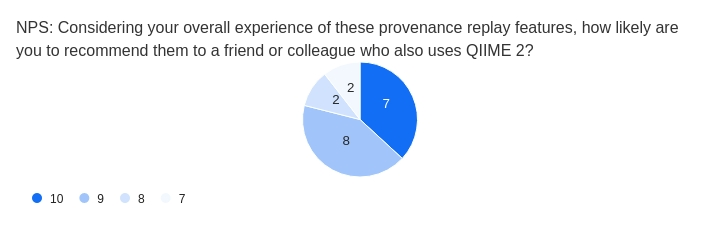
\includegraphics[width=\textwidth]{figures/NPS.jpg}
\caption[Pie chart of net promoter score responses]%
{Pie chart of net promoter score responses, showing seven responses at the
highest value (10), eight at the second highest (9), and two responses each at 8
and 7. No responses rated below 7.}
\label{fig:NPS}
\end{figure}

Though there is still considerable academic debate about the value and
limitations of NPS as a predictive measure \parencite[Table 1]{baehre_use_2022},
it is widely used and less frequently criticized as a measure of “how we are
doing right now”. Our high NPS seems to indicate that users believe this
software is currently worth recommending to others.

\subsection{Technology Acceptance Model (TAM) Results}

Provenance Replay also scored well on the Technology Acceptance Model
instruments. All PEOU questions were framed to ensure that increased ease of use
correlates with a higher numerical score (scaled from 1-7). We assume that all
response sentiment options are evenly distributed across the scale. Similarly,
all PU questions were framed to associate higher perceived usefulness with a
higher numerical score. (Table \ref{tab:scaled_likert_vals})

\begin{table}[htp]
        \begin{tabular}{|p{0.08\textwidth}|p{0.08\textwidth}|p{0.08\textwidth}|p{0.3\textwidth}|p{0.3\textwidth}|}
        \hline
        Score & From  & To    & Response          & Verbal Interpretation \\ \hline
        1     & 1     & 1.857 & Strongly Disagree & Very low              \\
        2     & 1.857 & 2.714 & Disagree          & Low                   \\
        3     & 2.714 & 3.571 & Somewhat Disagree & Somewhat Low          \\
        4     & 3.571 & 4.429 & Neither           & Neither               \\
        5     & 4.429 & 5.286 & Somewhat Agree    & Somewhat High         \\
        6     & 5.286 & 6.143 & Agree             & High                  \\
        7     & 6.143 & 7     & Strongly Agree    & Very high             \\ \hline
        \end{tabular}
    \caption[Scaled likert values for TAM interpretation]%
    {Scaled likert values evenly distribute the ranges to which we map our mean values}
    \label{tab:scaled_likert_vals}
\end{table}

All questions received mean scores of 5.36 or greater, indicating at least a
“high” PU or PEOU for all questions. One question had a median score of 5,
(“slightly agrees”) three had a median score of 7 (“strongly agrees”), and
the rest scored a median of 6 (“agrees”). Respondents rated Perceived Ease of
Use as “high”, with an overall mean of 5.82. Respondents rated Perceived
Usefulness as “high”, with an overall mean of 5.96.

Both PEOU and PU survey sections ended with “overall success” questions.
Respondents “strongly agree” that “Overall, [they] believe these features are
easy to use,” (mean 6.21, median 6) and “strongly agree” that “These features
are useful for me as a QIIME 2 user” (mean 6.16, median 7). With high PEOU and
POU, respondents indicate a positive general attitude toward using Provenance
Replay.

\subsection{Participant Technology Use and Attitude}

According to the TAM, external variables are contributing factors in PEOU and
PU. We gathered information about respondent technology use and attitude, as
these seem likely to influence perceptions and by extension likelihood of
technology uptake.

Respondents had very high rates of command shell use (mean 6.53, median 7), high
average comfort using programming languages (mean, 5.79, median 7, variance
relatively high at 2.38), high average comfort using QIIME 2 (mean 5.84, median
6), and somewhat high average comfort using QIIME 2’s provenance tracking
features (mean 4.68, median 5). Participants were somewhat satisfied with their
current QIIME 2 analysis workflow (mean 4.74, median 5.00), and somewhat agreed
that QIIME 2’s existing provenance tracking features are a useful tool in their
current analysis workflow (mean 4.95, median 5.00).

Respondents reported a very high level of enjoyment in learning to use new
computational tools (mean 6.53, median 7), and somewhat agreed that it is
generally easy for them to learn to use them (mean 5.21, median 5). They agreed
that they “enjoy using QIIME 2” (mean 5.95, median 6), and agreed that it is
generally easy for them to learn new things in QIIME 2. 

Overall, our cohort self-reports as highly computationally inclined, with
attitudes and beliefs about themselves that seem likely to encourage the
adoption of new technologies. This should be taken into account when considering
the strong NPS and TAM results.

\subsection{Feature Use and Rankings}

When asked to select all features they expected to incorporate into their
analyses:

\begin{itemize}
    \item 84\% of respondents believed they would use provenance replay to generate citations from their analyses
    \item 84\% of respondents believed they would generate new replay scripts from analysis results
    \item 74\% of respondents believed they would use QIIME 2’s existing provenance tracking features (including q2view provenance graphs)
    \item 32\% of respondents believed they would use Checksum Validation
\end{itemize}

These results are promising, indicating that a significant majority of
respondents believe the core replay tools implemented here will become part of
their QIIME 2 workflow.

A second question asked respondents to rank these four features in order of
value, where 1 represents the most valuable and four represents the least
valuable. Checksum Validation was \textit{by far} perceived as the least valuable feature
to our respondents (mean 3.67, median 4.00), while the three other features
clustered around 2, indicating a relatively even distribution of preference
between these three features, with provenance replay rating slightly higher than
the others, and citation replay slightly lower.

A second question asked respondents to rank these four features in order of
value, where 1 represents the most valuable and four represents the least
valuable. Checksum Validation was by far perceived as the least valuable feature
to our respondents (mean 3.67, median 4.00), while the three other features
clustered around 2, indicating a relatively even distribution of preference
between these three features, with provenance replay rating slightly higher than
the others, and citation replay slightly lower. (Table \ref{tab:feature_rankings})

\begin{table}[htp]
    \centering
    \begin{tabular}{|p{0.3\textwidth}|p{0.1\textwidth}|p{0.1\textwidth}|p{0.1\textwidth}|}
    \hline
    Feature             & Mean & Median & SD  \\ \hline
    Provenance Replay   & 1.83 & 1.5    & .96 \\
    Provenance Tracking & 2.11 & 2      & .94 \\
    Citation Replay     & 2.39 & 2      & .89 \\ \hline
    \end{tabular}
    \caption[Respondent rankings of feature value]%
    {Rankings of feature value were tightly clustered around the center for the
    three better-performing features. Checksum validation, not included here,
    was clearly the least valued feature. Complete results are available in
    Appendix I.}
    \label{tab:feature_rankings}
\end{table}

\subsection{Potential confounders}

Confounding effects may exist. Many study participants were recruited from
research groups with professional associations with our laboratory group. The
popularity of the QIIME 2 Platform might convey an inflated sense of value. The
moderator’s role as developer may complicate participants’ ability to share
negative feedback. Participants might believe that by participating in the
demonstration they have received early access to tools that might benefit their
work. In all of these, agreeableness or perceived authority could drive
acquiescence bias, inflating our TAM scores and contributing to our very high
NPS.

Provenance Replay is available to users free of charge. The impact of cost on
PEOU is beyond the scope of this study, but could be an interesting topic for
further research. I have been unable to identify academic publications
benchmarking NPS when applied to Free and Open Source Software (FOSS) like QIIME
2 and Provenance Replay, but it seems reasonable to believe that free products
might also be more likely to receive higher than average NPS or TAM scores.

Finally, these scores are all based on a prepared demonstration of a product
pre-installed in a working computing environment. Though I have made best
efforts to package and document the software to make installation and use
straightforward, all survey metrics, and Perceived Ease of Use especially, could
shift dramatically if users have a different experience working with the
software independently than they did while it was demonstrated by its developer.
Time and recruitment constraints made hands-on sessions unfeasible, but further
work would benefit from reporting based on active software use.


\section{Focus Groups and feature elicitation}

Our primary goal in conducting focus groups was to provide open enough lines of
communication for people to freely share experiences, preferences, and ideas for
how Provenance Replay can be improved or extended to meet their needs most
effectively. Deriving meaning from loosely structured conversations is subject
to significant interpretive bias, but I have done my best to value different
types of feedback equally. Each recording was reviewed in full, and any
statements that I felt were relevant to the current usage of QIIME 2’s
provenance capture tools, the demonstrated state of Provenance Replay, or
potential future development of Provenance replay were noted. 

These notes took two primary forms, often used in parallel. In the first, I
attempted to capture the core intent of the statement in paraphrase, recording
the paraphrased statement if it was novel, or incrementing a counter next to an
appropriate existing paraphrase if one existed. For example, three people
expressed that they “like the citation feature.” I recorded the paraphrase with
a 1 counter when I first encountered the sentiment, and simply incremented the
counter on the second and third occurrences. This served the purpose of grouping
and quantifying similar sentiments, which made it much easier to categorize
statements and derive meaning from the full corpus. The two most popular
statements received four mentions each, five statements received three mentions,
four statements received two mentions, and twenty-one were mentioned only once.

In the second form, I recorded a paraphrase and a counter, and transcribed a
representative quote from the statement. These quotes attempted to be minimal
while preserving the full sentiment of the speaker, and serve two useful
purposes. First, they may provide different levels of emphasis, perspectives, or
motivations provided by participants whose core intent I categorized within the
same paraphrase. Second, they often provide compelling statements about the user
experience that are not adequately represented by a paraphrase.

Once enumerated, the paraphrased statements were grouped into categories
according to my perception of their relatedness to one another. This grouping
was done unsystematically and post facto, and is a potential source of bias or
misinterpretation, but I believe it served the practical need to distill four
hours of conversation into meaningful units for discussion. These groupings will
be the foci of the subsections that follow, which have been loosely ordered in
terms of occurrence frequency. Groups with the highest mean frequency per
paraphrase come first, and groups with lower frequency of expression follow. I
have given thorough treatment to the most compelling groups, while being much
more selective in choosing content I believe to be interesting or valuable from
the others. A broad selection of paraphrases, counts, and quotations is included
in Appendix I.

% TODO: Appendix ref ^

Quotes and paraphrases alike are shared here with no identifying information,
for the protection of the privacy of our participants.

\subsection{Availability/inclusion in the platform}

Questions and statements about the inclusion of provenance replay features in
core components of the QIIME 2 platform were the most frequent statements. These
ranged in strength from questions (e.g. "Is this ever going to become part of
QIIME?") through strong statements:

\begin{quote}
We shouldn't have to know [Provenance Replay] exists to go looking for it and
download it. It would be nice if it were either part of QIIME 2 or comes along
with it as a fellow traveler, like 'hey, it's right here if you need it!'
\end{quote}

\noindent The three ideas/questions I tracked in this category were:

\begin{table}[htp]
    \centering
    \begin{tabular}{|p{0.6\textwidth}|p{0.08\textwidth}|}
    \hline
    Intent                                                  & Count \\ \hline
    Provenance Replay should be included in QIIME 2         & 4     \\
    Provenance Replay features should be included in q2view & 3     \\
    Is this software available now?                         & 3     \\ \hline
    \end{tabular}
    \caption[Focus Group discussions of Provenance Replay's inclusion in QIIME 2]%
    {Paraphrased ideas/questions about provenance replay’s availability,
    alongside the number of times they were expressed}
    \label{tab:feature_rankings}
\end{table}

The three requests for information about current availability were relatively
neutral, expressing general curiosity or some desire to use.

Two of the expressions that Replay should be included in QIIME 2 were general
questions, one was a simple statement that it should be included, and one was
the blockquote above. My interpretation is that generally these features were
desirable, and, critically, that inclusion would meaningfully reduce barriers to
use.

The statements about inclusion in q2view, though less frequent, were more
targeted/motivated by personal experience - expressed more as active feature
requests than as curiosities. Strongly expressed feedback like this seems more
valuable to me, and though there are significant technical barriers to including
Provenance Replay in q2view, it is work that I believe should be considered
seriously. 

\begin{quote}
I don't know if it's possible and how easy it would be, but.... would it be...
some magical way where you have something like this where I have my [q2view]
provenance graph and I click and I say 'Well, this is the thing I want to
reproduce - go reproduce it, or give me a script, or whatever'
\end{quote}

\noindent This is a relatively straightforward feature request, based on the user
imagining their own workflow, and seems like a reasonable expectation from a
tool capable of visualizing provenance data.

\begin{quote}
I'm trying to think about talking to people about analyses. Often, I'm like
Okay, here's your qzv or whatever - go to view.qiime2.org and drag-and-drop
it... If replay could be hooked into view.qiime2.org so that when you're viewing
an artifact you could click something and say 'OK, generate the script for this
thing that I'm viewing' that would be great because then when I delivered the
artifact to somebody that I'd done an analysis for, that would be the entire
thing. It would be everything in one place and it wouldn't have to be an 'also,
I'm sending you the scripts'
\end{quote}

\noindent This quote expresses that the feature request would reduce friction in
collaboration and communication. Interestingly, it also makes concrete an idea
expressed in the abstract by the same speaker during a different part of the
discussion:

\begin{quote}
I feel like this really in some ways fulfills the promise of the QIIME 2
provenance, which is 'we're carrying the provenance with the artifact, so if you
have the artifact you know how you got it.' and that's a wonderful idea, which
so far I haven't been able to make use of. but this, I think, really makes this
actionable.
\end{quote}

\noindent These statements, taken together, show deep insight into one strength of QIIME
2’s decentralized approach to provenance tracking, and support my belief that
inclusion of replay features in q2view could go a long way toward reducing
operational and communication barriers to reproducibility. 

Inclusion in q2view could provide a secondary benefit by encouraging the use of
QIIME 2 artifacts as a de facto means of sharing information on QIIME 2 analyses.

\begin{quote}
I'm working on a meta-analysis, and I'm collecting data from all sorts of
different published studies. If data were published as QIIME artifacts with
provenance (with provenance replay), it would make it so much easier for me to
reprocess all of the data in the same way the original authors did. They did
publish their methods, they do have details, but it would be so much easier for
me to work things out without me having to email them all the time.
\end{quote}

\noindent There are some privacy concerns associated with this approach (e.g. in the fact
that QIIME 2 Results contain study metadata), but with good privacy/data hygiene
practices in place, it could reduce the communication costs of study
reproduction on both authors and study reproducers.

\subsection{Usability and enhancements to q2view}
\label{section:q2view_enh}

The in-browser provenance graph viewer provided by q2view (hosted at
view.qiime2.org) is a widely-used tool for interrogating the history of QIIME 2
analyses. Participants mentioned its use in conjunction with troubleshooting
errors for themselves and other users, finding specific parameters or semantic
type information from old analyses, identifying which artifacts predated some
specific result, and even deciding whether preliminary analyses must be modified
or re-run entirely. It was used to answer computational questions and biological
questions, and was used by a QIIME 2 forum moderator to help identify issues in
forum participant data.

Given its broad use, I was surprised by the lightly critical nature of comments
about the tool. Three users expressed that familiar QIIME 2 interface formats
(e.g. q2cli scripts) might improve readability over q2view. 

\begin{quote}
Sometimes it's hard for me to look at the provenance [in q2view] and understand
what it's saying, but if I could turn it into a script and look at the
commands.... I'm really familiar with those CLI commands.
\end{quote}

\noindent Another user expressed that they struggled to interact with the small size and
density of the nodes in the provenance graph, and that therefore, “it's great
for record-keeping... but interaction is limited.” Two insightful participants
noted that the searchability of scripts or notebooks can make them more
effective platforms for learning specific things about an analysis. Inclusion of
replay tools or a fulltext search bar into q2view could help alleviate these
issues significantly. Overall, this category seems to indicate that provenance
replay tools may be useful for users who need to learn from or interpret the
history of their QIIME 2 Results.

\subsection{Feature Recommendations}

Feature requests fit a relatively long-tailed distribution, with many feature
requests or preferences expressed only once. Four of the five listed in the
table below, however, were very popular during the focus groups. The two most
popular requests

The capture and reporting of provisioning parameters for running analyses on HPC
clusters or server systems was mentioned four times - a likely indication that
this is a point of friction for some QIIME 2 users, and that it is worth
considering for future development efforts. Reliably capturing data about
cluster provisioning from within the Python runtime might not be possible, but
creative solutions might exist. Discussed as possible future work in Section
5.1.3.

% TODO: Make this a labeled ref

Three users suggested that they would like QIIME 2 to support tracking/replay of
times when data is exported from QIIME 2 for analysis within outside software,
and optionally re-imported afterwards. This is out of scope for the current
implementation, but if a reasonable solution is discovered, this would greatly
improve the capacity of Provenance Replay to describe complex analyses in an
easily-interpretable fashion.

\begin{table}[htp]
    \centering

    \begin{tabular}{|p{0.78\textwidth}|p{0.08\textwidth}|}
    \hline
    Intent                                                                  & Count \\ \hline
    Capture computational (provisioning) requirements - memory, cores, time & 4     \\
    Annotate points where analysis leaves/returns to QIIME 2                & 3     \\
    I like the citation feature                                             & 3     \\
    A methods manifest would be useful                                      & 2     \\
    Tools for managing software environments would be important             & 2     \\ \hline
    \end{tabular}

    \caption[Focus Group feature requests selected by popularity]%
    {The most popular feature suggestions alongside the number of times they
    were requested. All feature requests not included here or in Section \ref{section:q2view_enh}
    were suggested once.}
    \label{tab:feature_rankings}
\end{table}

The existing citation feature was popular, as was the idea of a “methods
manifest” (my term), which would provide an ordered, natural-language annotation
of the methods used, associated citations, and possibly references to software
versions or dependencies. This feature was an idea that arose during an early
focus group conversation, which I mentioned in later focus groups. The two
“mentions” by participants were strong approvals of the idea, as described by me
in response to the participant statements or questions.

\begin{quote}
You piqued my interest when you talked about the idea of a methods manifest,
because that's something that comes up all the time. The last role that I was
in, when we had some analyses that we did frequently, we had a methods text with
places where you fill in... what versions you used and what you used for this
parameter.... I'm really intrigued and enthusiastic... that this could maybe
help produce methods information.... the actual scripts are wonderful, but
they're for a different audience than trying to boil down 'what did I do' to
publish and so on.
\end{quote}

\noindent Further development of the idea will be required, but this idea is likely to be
targeted for future work.

Finally, tools for managing software environments were mentioned twice, with one
participant highlighting the fact that analyses might be conducted across
multiple different QIIME 2 versions as a possible challenge to Replay. Two
approaches were proposed, both of which are in consideration for future work.
"the easiest option would be saying what versions you need and how to install
them" is a documentation-oriented approach, leaving environment construction and
application to the user. "We should have something that will configure your
environment based on... [recorded] dependencies" presents a more robust
approach, potentially usable for fully-automated replay workflows.
% etc.
                                        % Heading commands (in descending order):
                                        % \chapter
                                        % \section
                                        % \subsection
                                        % \subsubsection
                                        % \paragraph
                                        % \subparagraph
\iftoggle{sample}{%
  \chapter{This is a chapter-level heading}

\lipsum[1]

\section{This is the first section-level heading}

% Test single- and double-spacing around block quotes
Nam dui ligula, fringilla a, euismod sodales, sollicitudin vel, wisi. Morbi auctor
lorem non justo. Nam lacus libero, pretium at, lobortis vitae, ultricies et, tellus. Donec
aliquet, tortor sed accumsan bibendum, erat ligula aliquet magna, vitae ornare odio
metus a mi. Morbi ac orci et nisl hendrerit mollis. Suspendisse ut massa. Cras nec ante.
Pellentesque a nulla. Cum sociis natoque penatibus et magnis dis parturient montes,
nascetur ridiculus mus. Aliquam tincidunt urna. Nulla ullamcorper vestibulum turpis.
Pellentesque cursus luctus mauris.
\begin{quote}
Nulla malesuada porttitor diam. Donec felis erat, congue non, volutpat
at, tincidunt tristique, libero. Vivamus viverra fermentum felis. Donec
nonummy pellentesque ante. Phasellus adipiscing semper elit. Proin
fermentum massa ac quam. Sed diam turpis, molestie vitae, placerat
a, molestie nec, leo. Maecenas lacinia. Nam ipsum ligula, eleifend at,
accumsan nec, suscipit a, ipsum. Morbi blandit ligula feugiat magna.
Nunc eleifend consequat lorem. Sed lacinia nulla vitae enim. Pellentesque
tincidunt purus vel magna. Integer non enim. Praesent euismod nunc eu
purus. Donec bibendum quam in tellus. Nullam cursus pulvinar lectus.
Donec et mi. Nam vulputate metus eu enim. Vestibulum pellentesque
felis eu massa.
\end{quote}
Quisque ullamcorper placerat ipsum. Cras nibh. Morbi vel justo vitae lacus tincidunt
ultrices. Lorem ipsum dolor sit amet, consectetuer adipiscing elit. In hac habitasse
platea dictumst. Integer tempus convallis augue. Etiam facilisis. Nunc elementum
fermentum wisi. Aenean placerat. Ut imperdiet, enim sed gravida sollicitudin, felis
odio placerat quam, ac pulvinar elit purus eget enim. Nunc vitae tortor. Proin tempus
nibh sit amet nisl. Vivamus quis tortor vitae risus porta vehicula.

\subsection{This is the first sub-section-level heading}

% Make sure single- and double-spacing around blocks works with line breaks in the source
Nam dui ligula, fringilla a, euismod sodales, sollicitudin vel, wisi. Morbi auctor
lorem non justo. Nam lacus libero, pretium at, lobortis vitae, ultricies et, tellus. Donec
aliquet, tortor sed accumsan bibendum, erat ligula aliquet magna, vitae ornare odio
metus a mi. Morbi ac orci et nisl hendrerit mollis. Suspendisse ut massa. Cras nec ante.
Pellentesque a nulla. Cum sociis natoque penatibus et magnis dis parturient montes,
nascetur ridiculus mus. Aliquam tincidunt urna. Nulla ullamcorper vestibulum turpis.
Pellentesque cursus luctus mauris.

\begin{quote}
Nulla malesuada porttitor diam. Donec felis erat, congue non, volutpat
at, tincidunt tristique, libero. Vivamus viverra fermentum felis. Donec
nonummy pellentesque ante. Phasellus adipiscing semper elit. Proin
fermentum massa ac quam. Sed diam turpis, molestie vitae, placerat
a, molestie nec, leo. Maecenas lacinia. Nam ipsum ligula, eleifend at,
accumsan nec, suscipit a, ipsum. Morbi blandit ligula feugiat magna.
Nunc eleifend consequat lorem. Sed lacinia nulla vitae enim. Pellentesque
tincidunt purus vel magna. Integer non enim. Praesent euismod nunc eu
purus. Donec bibendum quam in tellus. Nullam cursus pulvinar lectus.
Donec et mi. Nam vulputate metus eu enim. Vestibulum pellentesque
felis eu massa.
\end{quote}

Quisque ullamcorper placerat ipsum. Cras nibh. Morbi vel justo vitae lacus tincidunt
ultrices. Lorem ipsum dolor sit amet, consectetuer adipiscing elit. In hac habitasse
platea dictumst. Integer tempus convallis augue. Etiam facilisis. Nunc elementum
fermentum wisi. Aenean placerat. Ut imperdiet, enim sed gravida sollicitudin, felis
odio placerat quam, ac pulvinar elit purus eget enim. Nunc vitae tortor. Proin tempus
nibh sit amet nisl. Vivamus quis tortor vitae risus porta vehicula.

\subsubsection{This is the first sub-sub-section-level heading}

\lipsum[1]

\paragraph{This is the first paragraph-level heading}

\lipsum[1]

\subparagraph{This is the first sub-paragraph-level heading}

\lipsum[1]

\section{Citation examples}

The contents of this section differ depending on the bibliography settings, specifically whether the `usebiblatex' toggle is set to `true' or `false'.
\iftoggle{usebiblatex}{%
  This sentence shows citation with biblatex \parencite{searchinger_world_2013}.
  This is another sentence showing citation with biblatex \parencite{pathak_rural_2007}.
}{%
  This sentence shows citation with natbib \citep{pathak_rural_2007}.
  This is another sentence showing citation with natbib \citep{searchinger_world_2013}.
}

\section{Footnote examples}

This is a sentence followed by a footnote.\footnote{Mauris ut leo. Cras viverra metus rhoncus sem. Nulla et lectus vestibulum urna fringilla ultrices. Phasellus eu tellus sit amet tortor gravida placerat. Integer sapien est, iaculis in, pretium quis, viverra ac, nunc. Praesent eget sem vel leo ultrices biben- dum. Aenean faucibus. Morbi dolor nulla, malesuada eu, pulvinar at, mollis ac, nulla.}
This is another sentence followed by a footnote.\footnote{Mauris ut leo. Cras viverra metus rhoncus sem. Nulla et lectus vestibulum urna fringilla ultrices. Phasellus eu tellus sit amet tortor gravida placerat. Integer sapien est, iaculis in, pretium quis, viverra ac, nunc. Praesent eget sem vel leo ultrices biben- dum. Aenean faucibus. Morbi dolor nulla, malesuada eu, pulvinar at, mollis ac, nulla.}

\section{Block quote example}

The following is a block quote:

\begin{quote}
\lipsum[1-2]
\end{quote}

\section{Endnote examples}

Endnotes appear in a separate section after chapters and before the reference list.
This is a sentence followed by a endnote.\pagenote{Mauris ut leo. Cras viverra metus rhoncus sem. Nulla et lectus vestibulum urna fringilla ultrices. Phasellus eu tellus sit amet tortor gravida placerat. Integer sapien est, iaculis in, pretium quis, viverra ac, nunc. Praesent eget sem vel leo ultrices biben- dum. Aenean faucibus. Morbi dolor nulla, malesuada eu, pulvinar at, mollis ac, nulla.}
This is another sentence followed by a endnote.\pagenote{Mauris ut leo. Cras viverra metus rhoncus sem. Nulla et lectus vestibulum urna fringilla ultrices. Phasellus eu tellus sit amet tortor gravida placerat. Integer sapien est, iaculis in, pretium quis, viverra ac, nunc. Praesent eget sem vel leo ultrices biben- dum. Aenean faucibus. Morbi dolor nulla, malesuada eu, pulvinar at, mollis ac, nulla.}
And here is a really long endnote to show formatting across several pages.\pagenote{\expandafter\lipsum[1-6]}

\section{Table example}

See table \ref{table\arabic{tablecounter}} for an example of a table.
Place macros inside captions using \string\macrocapwrap.
See table \ref{table\arabic{tablecounter}} for a demonstration.

\begin{table}[h] % Table float
\caption{Here is a table caption that is especially long to show what happens when it extends to more than one line in the table of contents}
\label{table\arabic{tablecounter}}
\begin{tabu}{l c c} \\ \hline
Column1 & Column2 & Column3 \\ \hline
Row1 & 2.0 & 3.0 \\
Row2 & 2.0 & 3.0 \\
Row3 & 7.0 & 8.0 \\ \hline
\end{tabu}
\legend{\emph{Source}: Here is a source note that is especially long to show what happens when it extends to more than one line.}
\legend{\emph{Note}: Here is a note that is especially long to show what happens when it extends to more than one line.}
\end{table}
\refstepcounter{tablecounter}

\begin{table}[h] % Table float
\caption{This table caption refers to another caption: see figure \macrocapwrap{\ref{figure1}} }
\label{table\arabic{tablecounter}}
\begin{tabu}{l c c} \\ \hline
Column1 & Column2 & Column3 \\ \hline
Row1 & 2.0 & 3.0 \\
Row2 & 2.0 & 3.0 \\
Row3 & 7.0 & 8.0 \\ \hline
\end{tabu}
\end{table}
\refstepcounter{tablecounter}

\section{Figure example}

See figure \ref{figure\arabic{figurecounter}} for an example of a figure.

\begin{figure}
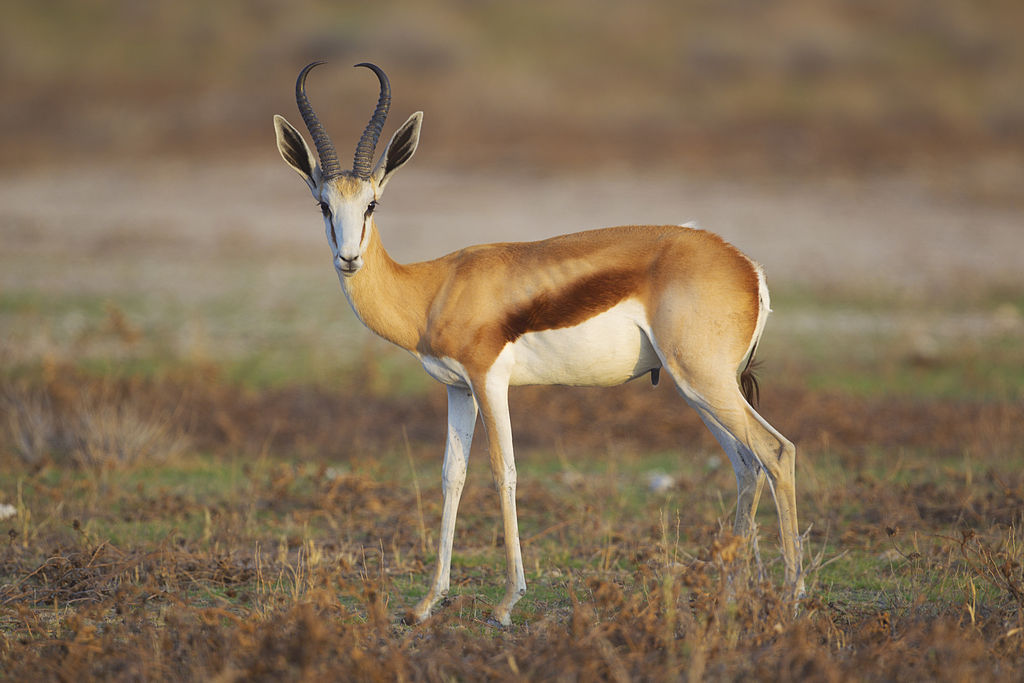
\includegraphics[width=\maxwidth{\textwidth}]{src/sample/antidorcas.jpg}
\caption{Antidorcas marsupialis, male}
\label{figure\arabic{figurecounter}}
\legend{\emph{Source}: \iftoggle{usebiblatex}{\textcite{krishnappa_adult_2012}}{\citet{krishnappa_adult_2012}}}% See: https://upload.wikimedia.org/wikipedia/commons/8/89/Antidorcas_marsupialis%2C_male_%28Etosha%2C_2012%29.jpg
\legend{\emph{Note}: Here is a note that is especially long to show what happens when it extends to more than one line.}
\end{figure}
\refstepcounter{figurecounter}
\clearpage
\section{Math examples}

This section contains some math-heavy text adapted from \iftoggle{usebiblatex}{\textcite{dwilkins1995}}{\citet{dwilkins1995}}.
In non-relativistic wave mechanics, the wave function $\psi(\mathbf{r},t)$ of a particle satisfies the Schrödinger Wave Equation
%
\begin{equation}
 i\hbar\frac{\partial \psi}{\partial t}
  = \frac{-\hbar^2}{2m} \left(
    \frac{\partial^2}{\partial x^2}
    + \frac{\partial^2}{\partial y^2}
    + \frac{\partial^2}{\partial z^2}
  \right) \psi + V \psi.
\end{equation}
%
It is customary to normalize the wave equation by
demanding that
%
\begin{equation}
\int \!\!\! \int \!\!\! \int_{\textbf{R}^3}
      \left| \psi(\mathbf{r},0) \right|^2\,dx\,dy\,dz = 1.
\end{equation}
%
A simple calculation using the Schr\"{o}dinger wave
equation shows that
%
\begin{equation}
\frac{d}{dt} \int \!\!\! \int \!\!\! \int_{\textbf{R}^3}
      \left| \psi(\mathbf{r},t) \right|^2\,dx\,dy\,dz = 0,
\end{equation}
%
and hence
%
\begin{equation}
\int \!\!\! \int \!\!\! \int_{\textbf{R}^3}
      \left| \psi(\mathbf{r},t) \right|^2\,dx\,dy\,dz = 1
\end{equation}
%
for all times~$t$. If we normalize the wave function in this
way then, for any (measurable) subset~$V$ of $\textbf{R}^3$
and time~$t$,
%
\begin{equation}
\int \!\!\! \int \!\!\! \int_V
      \left| \psi(\mathbf{r},t) \right|^2\,dx\,dy\,dz
\end{equation}
%
represents the probability that the particle is to be found
within the region~$V$ at time~$t$.

\begin{table}[h] % Table float
\caption{This caption has math characters that remain lowercase: \relax\macrocapwrap{$\psi(\mathbf{r},t)$} }
\label{table\arabic{tablecounter}}
\begin{tabu}{l c c} \\ \hline
Column1 & Column2 & Column3 \\ \hline
Row1 & 2.0 & 3.0 \\
Row2 & 2.0 & 3.0 \\
Row3 & 7.0 & 8.0 \\ \hline
\end{tabu}
\end{table}
\refstepcounter{tablecounter}
%
}{}
%%%%%%%%%%%%%%%%%%%%%%%%%%%%%%%%%%%%%%%
% Back matter
%%%%%%%%%%%%%%%%%%%%%%%%%%%%%%%%%%%%%%%
\SingleSpacing                          % Back matter should be single spaced
\AfterEndEnvironment{table}{\SingleSpacing} % Reset these environments
\AfterEndEnvironment{figure}{\SingleSpacing}
\AfterEndEnvironment{quote}{\SingleSpacing}
\AfterEndEnvironment{quotation}{\SingleSpacing}

\edef\defaulttolerance{\the\tolerance}
\tolerance 500                          % Increase tolerance to prevent material extending into margins
\hbadness 500

\iftoggle{useendnotes}{%                % If you're using endnotes, output them here
  \setsecnumdepth{none}                 % No section numbering in end notes
  \bookmarksetup{startatroot}           % Make Notes appear at root level of PDF bookmarks
  \phantomsection%                      % Need for hyperref
  \addcontentsline{toc}{chapter}{%      % Add a chapter-level heading for
    \hspace{-\cftchapterindent}%        %  Notes to the ToC
    \notesname%
  }%
  \renewcommand*{\notedivision}{%
    \chapter*{\notesname}%
  }
  \printpagenotes                       % Output the notes
  \setsecnumdepth{all}%                 % Turn section numbering back on after printing
}{}

\bookmarksetup{startatroot}
\chapter*{\bibheading}                  % In the running text, use a chapter-level heading
                                        % for the bibliography section
\phantomsection
\addcontentsline{toc}{chapter}{%        % In the TOC, add a custom chapter-level heading
  \hspace{-\cftchapterindent}%          % that will be flush against the left margin
  \bibheading%
}
%\phantomsection
%\addtocontents{toc}%                    % Add this 'mark' to TOC so subsequent pages use
%  {\protect\markboth{\bibheading}{Page}}%   the bibliography heading (unlikely since
%                                        %   the appendices follow quickly)
\iftoggle{usebiblatex}{%                % Output the bibliography
  \printbibliography[heading=none]      % Using a 'biblatex' package; do not let
                                        %   'biblatex' output a heading
}{%
  \renewcommand\bibsection{}            % Do not let 'natbib' output a heading
  \bibliographystyle{\natbibstyle}      % Using 'natbib' to print bibliography
  \bibliography{\bibfilename}
}

\appendix                               % Indicate start of appendices
                                        % Appendices are considered 'mainmatter' in this
                                        %   documentclass
\tolerance \defaulttolerance            % Set tolerance back to default
\hbadness \defaulttolerance

\addtocontents{toc}{\protect%           % Only include appendix title in table of contents
  \setcounter{tocdepth}{0}}%            %   and omit sub-headings
\renewcommand*{\chapnamefont}%          % Reset font for 'Appendix' in chapter titles
    {\normalfont\MakeTextUppercase}
\makeatletter                           % Clear page after printing appendix title
  \renewcommand{\memendofchapterhook}%
  {%
    \clearpage
    \m@mindentafterchapter
    \@afterheading
  }
\makeatother

\phantomsection                         % Need '\phantomsection' to place hyperref
                                        %   bookmark more accurately
\addcontentsline{toc}{part}{Appendix}   %~Add "Appendix" to TOC here; comment out this
                                        %   line if you're not including appendices

%\phantomsection                        %!This is the one part of the template that I
%\addtocontents{toc}%                   %   could not get to work properly. After you
%  {\protect\markboth{APPENDIX}{Page}}  %   start listing appendices in the TOC,
                                        %   subsequent TOC pages should use "APPENDIX in
                                        %   the header instead of "CHAPTER"; however,
                                        %   this code will make "APPENDIX" appear on the
                                        %   the same page that the *first* appendix
                                        %   appears on. This problem won't affect most
                                        %   people, but if it affects you, uncomment
                                        %   these lines and move them below where
                                        %   the appendices are listed. Keep moving these
                                        %   lines down and checking the output until
                                        %   the TOC headers appear correctly

%\input{appendix1}                       %~Insert your appendices here; I recommend to use
%\input{appendix2}                       %   \input rather than \include for appendices.
%\input{appendix3}% etc.                 %   All heading commands are the same as above,
                                         %   e.g., \chapter, \section, etc.
\iftoggle{sample}{%
  \chapter{This is a chapter-level heading for an appendix}

\lipsum[1]

\section{This is the first section-level heading in the appendix}

\lipsum[1]

\subsection{This is the first sub-section-level heading in the appendix}

\lipsum[1]

\subsubsection{This is the first sub-sub-section-level heading in the appendix}

\lipsum[1]

\paragraph{This is the first paragraph-level heading in the appendix}

\lipsum[1]

\subparagraph{This is the first sub-paragraph-level heading in the appendix}

\lipsum[1] %
}{}

\backmatter                             % Start back matter according to documentclass
\makeatletter                           % Do not clear page after printing title for
  \renewcommand{\memendofchapterhook}%  %   biographical sketch
  {%
    \m@mindentafterchapter
    \@afterheading
  }
\makeatother

%\biographicalsketch{%                  %~Biographical Sketch is optional
%  \input{biography}%                   %<Enter the name of the .tex file containing your
%}%                                     %   biography or omit this line and type in
                                        %   your biography here (1 paragraph)
\end{document}
